% \documentclass[mat1, tisk]{fmfdelo}
\documentclass[fin1, tisk]{fmfdelo}
% Če pobrišete možnost tisk, bodo povezave obarvane,
% na začetku pa ne bo praznih strani po naslovu, …

%%%%%%%%%%%%%%%%%%%%%%%%%%%%%%%%%%%%%%%%%%%%%%%%%%%%%%%%%%%%%%%%%%%%%%%%%%%%%%%
% METAPODATKI
%%%%%%%%%%%%%%%%%%%%%%%%%%%%%%%%%%%%%%%%%%%%%%%%%%%%%%%%%%%%%%%%%%%%%%%%%%%%%%%

% - vaše ime
\avtor{Janez Podlogar}

% - naslov dela v slovenščini
\naslov{Kontekstno-neodvisne gramatike za kodiranje in stiskanje podatkov}

% - naslov dela v angleščini
\title{Context-Free Grammars for Data Encoding and Compression}

% - ime mentorja/mentorice s polnim nazivom:
%   - doc.~dr.~Ime Priimek
%   - izr.~prof.~dr.~Ime Priimek
%   - prof.~dr.~Ime Priimek
%   za druge variante uporabite ustrezne ukaze
\mentor{prof.~dr.~Ljupčo Todorovski}
% \somentor{...}
% \mentorica{...}
% \somentorica{...}
% \mentorja{...}{...}
% \somentorja{...}{...}
% \mentorici{...}{...}
% \somentorici{...}{...}

% - leto diplome
\letnica{2024} 

% - povzetek v slovenščini
%   V povzetku na kratko opišite vsebinske rezultate dela. Sem ne sodi razlaga
%   organizacije dela, torej v katerem razdelku je kaj, pač pa le opis vsebine.
\povzetek{Definiramo podrazred kontekstno-neodvisnih gramatik, imenovan dopustne gramatike.
Nizu $w$ iz dane abecede priredimo dopustno gramatiko $G_w$, katere jezik je $\{ w \}$.
Predstavimo dva razreda prirejanja dopustne gramatike nizu in za vsakega podamo algoritem.
Za stiskanje niza $w$ z binarnim kodiranjem prepisovalnih pravil dopustne gramatike 
$G_w$ analiziramo odvečnost in pokažemo, da je takšno stiskanje univerzalna koda.}

% - povzetek v angleščini
\abstract{We define a subclass of context-free grammars, called admissable grammars. For each
string $w$ from a given alphabet, we assign an admissable grammar $G_w$, such that its language
is $\{ w \}$. We introduce two classes of assigning an admissable grammars to a string and 
provide an algorithm for each. We analyze the redundancy in lossless compression of a string $w$
using a binary encoding of the production rules of tje admissable grammar $G_w$ and demonstrate 
that such compression constitutes a universal code.
}

% - klasifikacijske oznake, ločene z vejicami
%   Oznake, ki opisujejo področje dela, so dostopne na strani https://www.ams.org/msc/
\klasifikacija{68P30, 68Q42, 94A15}
% 68P30 - Coding and information theory (compaction, compression, models of communication,
% encoding schemes, etc.
% 68Q42 - Grammars and rewriting systems
% 94A15 - Information theory (general)


% - ključne besede, ki nastopajo v delu, ločene s \sep
\kljucnebesede{kontekstno-neodvisna gramatika\sep stiskanje podatkov\sep teorija informacij\sep
stiskanje brez izgube\sep univerzalna koda}

% - angleški prevod ključnih besed
\keywords{context-free grammar\sep data compression\sep information theory\sep lossless compression\sep universal code}

% - angleško-slovenski slovar strokovnih izrazov
\slovar{
% \geslo{angleški izraz}{slovenski izraz}
\geslo{admissable grammar}{dopustna gramatika}
\geslo{alphabet}{abeceda}
\geslo{channel}{kanal}
\geslo{code}{kod}
\geslo{concatenation}{stikanje}
\geslo{context-free grammar}{kontekstno-neodvisna gramatika}
\geslo{data compression}{stiskanje podatkov}
\geslo{decoder}{dekodirnik}
\geslo{discrete memoryless source}{diskretni vir brez spomina}
\geslo{encoder}{kodirnik}
\geslo{encoding}{kodiranje}
\geslo{encryption}{šifriranje}
\geslo{entropy}{entropija}
\geslo{enumerate encoding}{leksikografsko kodiranje}
\geslo{error correcting code}{kod za popravljanje napak}
\geslo{finite state source}{končni vir}
\geslo{formal grammar}{formalna gramatika}
\geslo{information source}{informacijski vir}
\geslo{information theory}{teorija informacij}
\geslo{irreducible grammar}{neskrčljiva gramatika}
\geslo{language over an alphabeth}{jezik na abecedi}
\geslo{left-total relation}{celovita relacija}
\geslo{lossless compression}{stiskanje brez izgube}
\geslo{lossy compression}{stiskanje z izgube}
\geslo{maximal pointwise redundancy}{maksimalna točkovna odvečnost}
\geslo{phrase structure grammar}{frazeološka strukturna gramatika}
\geslo{prefix}{predpona}
\geslo{production rules}{prepisovalno pravilo}
\geslo{reciever}{sprejemnik}
\geslo{redundancy}{odvečnost}
\geslo{total order}{linearna urejenost}
\geslo{unary coding}{eniško kodiranje}
\geslo{universal code}{univerzalna koda}
\geslo{unrestricted grammar}{neomejena gramatika}
}

% - ime datoteke z viri (vključno s končnico .bib), če uporabljate BibTeX
\literatura{literatura.bib}

%%%%%%%%%%%%%%%%%%%%%%%%%%%%%%%%%%%%%%%%%%%%%%%%%%%%%%%%%%%%%%%%%%%%%%%%%%%%%%%
% DODATNE DEFINICIJE
%%%%%%%%%%%%%%%%%%%%%%%%%%%%%%%%%%%%%%%%%%%%%%%%%%%%%%%%%%%%%%%%%%%%%%%%%%%%%%%

% naložite dodatne pakete, ki jih potrebujete

% Model komunikacije in končni vir/automat
\usepackage{tikz}
\usetikzlibrary{positioning, fit, calc, automata, arrows}

% Graf
\usepackage{tkz-graph,tkz-berge}

% Slike
\usepackage{float}
\usepackage{graphicx}
\graphicspath{{./images/}}

% Formalizacija primer:mors
\newcommand\Vtextvisiblespace[1][.3em]{%
  \mbox{\kern.06em\vrule height.3ex}%
  \vbox{\hrule width#1}%
  \hbox{\vrule height.3ex}}

\providecommand{\abs}[1]{\left\lvert #1 \right\rvert}

% Naravna števila
\newcommand{\N}{\mathbb{N}}

% Realna števila
\newcommand{\R}{\mathbb{R}}

% Verjetnost
\newcommand{\probP}{\text{I\kern-0.15em P}}

% Pričakovana vrednost
\newcommand{\E}{\mathbb{E}}

% Abeceda
\newcommand{\A}{\mathcal{A}}

% Podmnožica KNG
\newcommand{\G}{\mathcal{G}}

% \xRightarrow
\usepackage{mathtools}

% Za skrčitvena pravila
\theoremstyle{definition}
\newtheorem{pravilo}{Skrčitveno pravilo}

% deklarirajte vse matematične operatorje, da jih bo LaTeX pravilno stavil
% \DeclareMathOperator{\...}{...}

% vstavite svoje definicije ...
% \newcommand{\...}{...}

%%%%%%%%%%%%%%%%%%%%%%%%%%%%%%%%%%%%%%%%%%%%%%%%%%%%%%%%%%%%%%%%%%%%%%%%%%%%%%%
% ZAČETEK VSEBINE
%%%%%%%%%%%%%%%%%%%%%%%%%%%%%%%%%%%%%%%%%%%%%%%%%%%%%%%%%%%%%%%%%%%%%%%%%%%%%%%

\begin{document}

\section{Uvod}

Temeljni problem sporazumevanja je prenos sporočila od informacijskega vira do sprejemnika.
Privzemimo komunikacijski model prikazan na spodnji sliki, ki je prirejna po~\cite{Shannon1949}.
\tikzset{block/.style={draw, thick, text width=3cm, minimum height=1.5cm, align=center}, line/.style={-latex}}
\begin{figure}[H]
    % Enako kot Shannonov model z odstranjenim šumom
    \centering
    \scalebox{0.8}{
    \begin{tikzpicture}[scale=0.20]
        \node[block] (a) {informacijski vir};
        \node[block,right=of a] (b) {kodirnik};
        \node[block,right=of b, xshift=12mm] (c) {dekodirnik};
        \node[block,right=of c] (d) {sprejemnik};
        
        \draw[line] (a)-- (b);
        \draw[line] (b)-- (c) node[anchor=south,inner sep=2pt,midway] {kanal};
        \draw[line] (c)-- (d); 
    \end{tikzpicture}
    }
    \caption{Komunikacijski model}
\end{figure}

\emph{Informacijski vir} izbere želeno sporočilo iz množice vseh možnih sporočil.
\emph{Kodirnik} pretvori sporočilo v primereno obliko za prenos po \emph{kanalu}
do \emph{dekodirnika}, ki sporočilo pretvori v primerno obliko za \emph{sprejemnik}.
Spreminjanje zapisa sporočila imenujemo \emph{kodiranje}, sistemu pravil, po katerem se kodiranje
opravi, pa \emph{kod}. 

Besedilo, zapisano z pismenkami, je neberljivo za slepe osebe, saj je komunikacijski kanal v tem
primeru vid. Prav tako pisanega besedila v prvotni obliki ni mogoče poslati s telegrafom. 
V tem primeru je komunikacijski kanal žica in pismenke se po njej ne morejo sprehoditi. 
Najpomembnejši namen kodirnika je pretvorba sporočila v obliko, ki jo lahko pošljemo po kanalu.
V opisanih primerih je sporočilo, ki bi ga radi prenesli, zapisana v neprimerni obliki. V primeru
slebe osebe je potrebno besedilo zapisati z Braillovo pisavo, v primeru telegrafa pa je besedilo 
potrebno pretvoriti v električni signal, kot ilustrira naslednji primer.
\begin{primer}\label{primer:mors}
    \emph{Morsejeva abeceda} je kodiranje črk, številk in ločil s pomočjo 
    zaporedja kratkih in dolgih signalov. Določajo jo pravila:
    \begin{itemize}
        \item Dolžina kratkega signala je ena enota.
        \item Dolgi signal je trikrat daljši od kratkega signala.
        \item Razmik med signali znotraj črke je tišina dolžine kratkega signala.
        \item Razmik med črkami je tišina, dolga tri kratke signale oziroma en dolgi signal.
        \item Med besedami je tišina, dolga sedem kratkih signalov.
    \end{itemize}
    \begin{figure}[H]
        \centering
        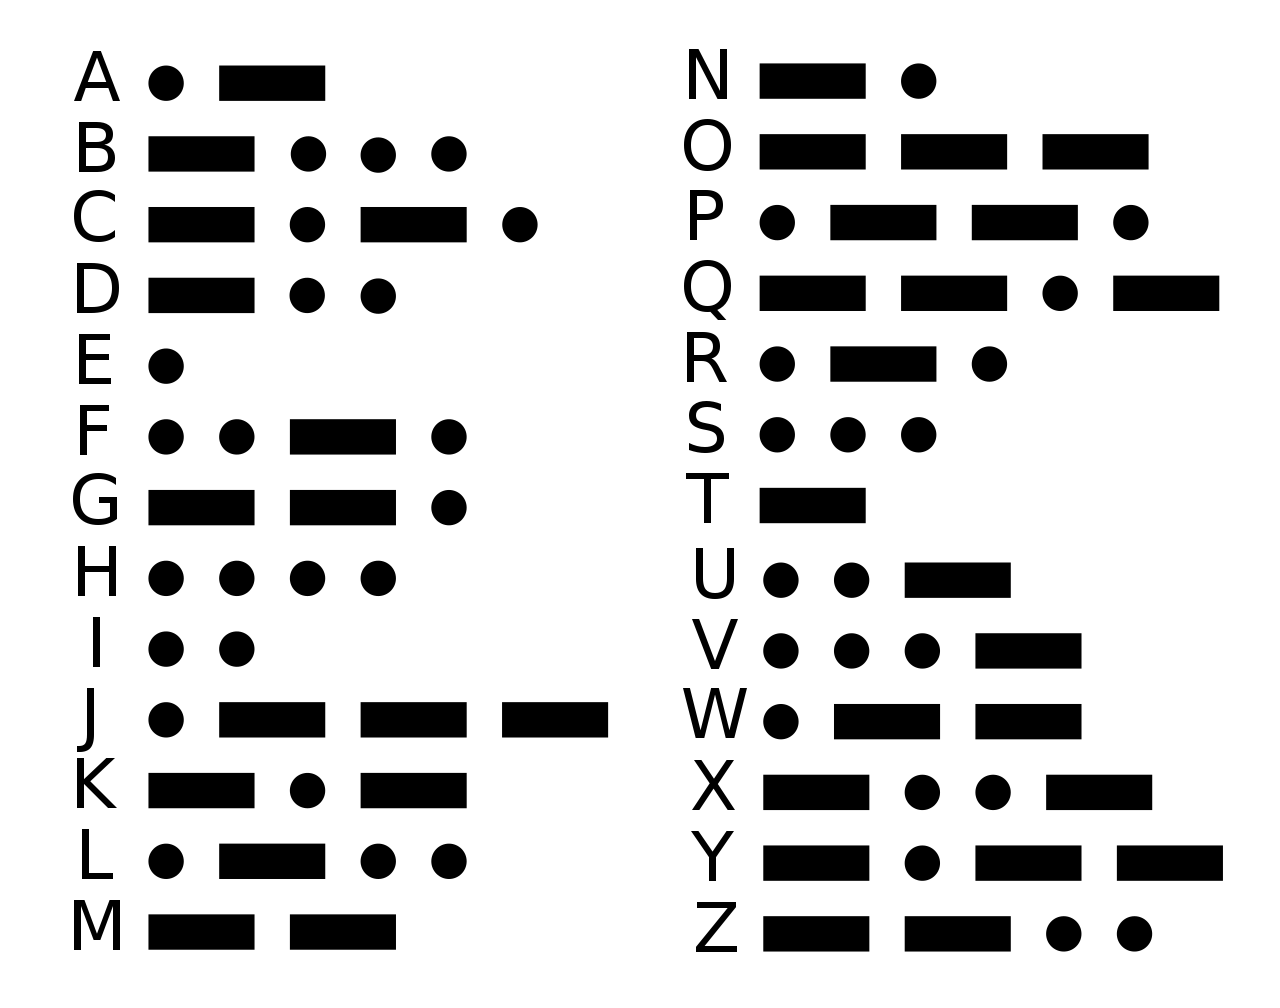
\includegraphics[width=5cm]{1280px-InternationalMorseCode.svg.png}
        \caption{Mednarodna Morsejeva abeceda, vzeta iz~\cite{morseletters}.}
        \label{fig:morse}
    \end{figure}
    Namen Morsejeve abecede je komunikacija preko telegrama, saj komunikacijski kanal dovoljuje 
    le električne signale in tišino med njimi.
\end{primer}

Od kodirnika zahtevamo več kot le pretvorbo v ustrezno obliko za prenos po kanalu.
Če imamo nezanesljiv kanal, se med prenosom po kanalu lahko pojavijo napake v sporočilu.
Kod za popravljanje napak nam omogoča, da za ceno daljšega sporočila popravimo napake, ki se 
pojavijo ob motnjah pri prenosu. %npr. Hammingova koda
Morda pa tudi nekoga tretjega zanima vsebina našega sporočila. Tedaj sporočilo kodiramo
tako, da ga lahko dekodirajo le pooblaščene osebe. Takšnemu kodiranju pravimo
šifriranje. Šifriranje ne preprečuje dostopa do kodiranega sporočila, ampak onemogoča pravilno
dešifiranje oziroma razumevanje vsebine prestrezniku. %npr Cezarjeva šifra
Eden izmed namenov kodiranja je tudi doseči jedernatost sporočila. Stiskanje podatkov 
je zapis informacij sporočila v zgoščeni obliki. Z uporabo lepih lastnosti sporočila, ga lahko
učinkoviteje prenesemo in porabimo manj prostora. Ena od takih lastnosti je statistična struktura
jezika. Uporabimo jo v Morsejevi abecedi, kjer imajo črke z višjo frekvenco (v angleškem jeziku) 
krajši zapis. %npr. Huffmanovo kodiranje

V delu bomo preučevali metode kodiranja, ki izkoriščajo prisotnost ponavljajočih se vzorcev
v sporočilu. Zanimalo nas bo stiskanje preko \emph{gramatike}, več o drugih metodah pa najdemo 
v~\cite{Sayood2017}. Gramatika ali slovnica je nabor pravil, ki jih mora stavek 
upoštevati, da je ``pravilen''. Pri stiskanju podatkov nas zanimajo \emph{formalne gramatike}, 
ki jih razumemo kot nabor prabil za generiranje zaporedja črk. Zaporedje črk želimo 
stisniti preko zgoščenega nabora pravil, ki generirajo dano zaporedje.

\begin{primer}
    \label{primer:motivacija}
    Poglejmo niz $w =\mathit{cababcccababcccab}$.
    Opazimo, da se v nizu ponovita vzorca $\mathit{ab}$ in $\mathit{ccc}$. Uvedemo novi oznaki
    $A = \mathit{ab}$ in $B = \mathit{ccc}$. Sedaj zapišemo niz $w$ kot
    \[
        w = \mathit{cAABAABA}.
    \]
    Uvedemo novo oznako $C = \mathit{AAB}$
    in zapišemo $w$ kot
    \[
        w = \mathit{cCCA}.
    \]
    Prvotni niz smo z novimi oznakami skrajšali. Kot bomo videli, smo niz $w$ pretvorili v 
    formalno gramatiko s pravili
    \begin{align*}
        & S  \rightarrow \mathit{cCCA}, \\
        & A  \rightarrow \mathit{ab}, \\
        & B  \rightarrow \mathit{ccc}, \\
        & C  \rightarrow \mathit{AAB}.
    \end{align*}
\end{primer}

\section{Osnovni pojmi}

\subsection{Jezik na abecedi}
Gradnik besedila je abeceda. To je množica črk, ki ponavadi predstavljajo zvoke v govorjenem
jeziku. Za nas bo abeceda množica veljavnih črk jezika.

\begin{definicija}
    \emph{Abeceda} je končna neprazna množica. Elementom abecede pravimo \emph{črke}.
    Za vsak $\ell > 0$ rekurzivno definiramo \emph{množico vseh nizov abecede $\A$ dolžine 
    $\ell + 1$}
    \begin{gather*}
        \A^0 = \{ \varepsilon \}, \\
        \A^{\ell+1} = \{ wa \mid w \in \A^{\ell} \text{ in } a \in \A \},
    \end{gather*}
    kjer $\varepsilon$ imenujemo \emph{prazen niz}.
    \emph{Množica vseh končnih nizov abecede $\A$} je
    \[
        \A^* = \bigcup_{\ell \geq 0} \A^\ell
    \]
    in \emph{množica vseh končnih nizov abecede $\A$ brez praznega niza} je
    \[
        \A^+ = \A^* \setminus \{ \varepsilon \}.
    \]
    \emph{Jezik na abecedi} $\A$ je poljubna podmnožica množice $\A^*$. 
    \emph{Dolžino niza w} označimo z $\abs{w}$ in je enaka številu črk v nizu $ w \in \A^* $.
\end{definicija}

\begin{definicija}
    Naj bo $\A$ abeceda in $*$ binarna operacija na $\A^*$ tako, da je $\varepsilon$ 
    nevtralni element in za niza $ w, u \in \A^* $ velja
    \[
        w*u = w_1w_2 \cdots w_nu_1u_2 \cdots u_m,
    \]
    kjer sta $w_1w_2 \cdots w_n$ in $u_1u_2 \cdots u_m$ predstavitvi nizov $w$ in $u$ s črkami
    abecede $\A$. Operacijo $*$ imenujemo \emph{stikanje}. Simbol $*$ spustimo in 
    krajše pišemo $wu$.
\end{definicija}

\begin{opomba}
    Stikanje je asociativna operacija. Torej je $(\A^*, *)$ monoid in $(\A^+, *)$ polgrupa.
\end{opomba}

\begin{definicija}
    Naj bo $w \in \A^*$ in $w = w_1w_2 \cdots w_n$ predstavitvi niza $w$ s črkami abecede 
    $\A$. \emph{Frekvenca črke $s$ v nizu $w$} je
    \[
        f(s|w) = \abs{ \bigl\{ i \in \{1, 2 \cdots, n\} \colon w_i = s \bigr\} }.
    \]
\end{definicija}

\begin{definicija}
    Niz $u \in \A^+$ je \emph{predpona} niza $w \in \A^+$, če $\exists v \in \A^*$, da je
    $uv = w$.
\end{definicija}

\begin{primer}\label{primer:string}
    Za abecedo $\A = \{ a,b,c \}$ so $\mathit{ab} \in \A^2$, $\mathit{abccc} \in \A^5$
    in $\mathit{cababcccababcccab} \in \A^{17}$ končni nizi abecede $\A$.
    Niz $\mathit{ab}$ je predpona niza $\mathit{abccc}$.
\end{primer}

\subsection{Kodiranje sporočila}

Kodiranje sporočila je spreminjanje zapisa sporočila po sistemu pravil, ki ga imenujemo kod. Kod
bomo podali s preslikavo.

\begin{definicija}
    \emph{Kodna preslikava} je injektivna preslikava $ \kappa \colon \A^*_s
    \to \A_c^* $, kjer imenujemo $\A_s$ \emph{izvorna abeceda}, $\A_c$ 
    \emph{kodna abeceda} in $\kappa(w)$ \emph{koda niza $w$}. 
    \emph{Dekodna preslikava} je preslikava $ \delta \colon C \subseteq \A^*_c 
    \to \A_s^* $, da velja
    \[
        \forall w \in \A_s^* \colon \delta(\kappa(w)) = w.
    \]
\end{definicija}

\begin{primer}
    Formalizirajmo Morsejevo abecedo iz primera~\ref{primer:mors}. Abecedi sta
    \[
        \A_s = \{ \text{A}, \text{B}, \ldots, \text{Z} \}
        \cup \{ \Vtextvisiblespace[5pt] \}, \quad
        \A_c = \{ \cdot ,-, \Box \},
    \]
    kjer je \Vtextvisiblespace[5pt] presledek, $cdot$ kratki signal, $-$ dolgi signal in $\Box$ 
    kratka enota tišine. Definiramo kodno preslikavo črk abecede 
    $\kappa_s \colon \A \to \A_c^*$, ki vsaki črki iz abecede $\A_s$ priredi niz črk 
    kodne abecede $\A_c$. Predpis preslikave $\kappa_s$ je določen na sliki~\ref{fig:morse}.
    Presledek \Vtextvisiblespace[5pt] kodiramo v eno kratko enoto tišine
    \[
        \kappa_s(\Vtextvisiblespace[5pt]) = \Box.
    \]
    Za niz $w = a_1a_2 \ldots, a_n \in \A^*$ kodno preslikavo $\kappa$ definiramo po črkah
    \[
        \kappa(w) = \kappa_s(a_1) \Box\Box\Box \kappa_s(a_2) \Box\Box\Box \cdots 
        \Box\Box\Box \kappa_s(a_n).
    \]
    Poglejmo dve kodiranji
    \begin{gather*}
        \kappa(\text{SOS}) = \phantom{} \cdot\Box\cdot\Box\cdot \Box\Box\Box -\Box-\Box- 
        \Box\Box\Box \cdot\Box\cdot\Box\cdot \phantom{}, \\
        \kappa(\text{ET\Vtextvisiblespace[5pt]TU}) = \phantom{} \cdot \Box\Box\Box - \Box\Box\Box
        \Box \Box\Box\Box - \Box\Box\Box \cdot\Box\cdot\Box- \phantom{}.
    \end{gather*}
    Recimo, da smo prejeli sporočilo, a se je pošiljatelj zmotil in je namesto kode,
    ki bi se dekodirala v
    \[
        \delta(\phantom{} -\Box-\Box\cdot\Box- \Box\Box\Box \cdot \Box\Box\Box -\Box\cdot\Box\cdot \phantom{}) = \text{QED},
    \]
    poslali kodo
    \[
        \phantom{} -\Box-\Box\cdot\Box-\Box- \Box\Box\Box \cdot \Box\Box\Box -\Box\cdot\Box\cdot \phantom{}.
    \]
    Sporočila ne znamo dekodirati, saj se ne nahaja v domeni $ C $ dekodne preslikave $ \delta $.
\end{primer}

Kodiranje z namenom krajšanja zapisa sporočila imenujemo \emph{stiskanje podatkov}.

\begin{definicija}
    \emph{Stiskanje} je kodna preslikava $\kappa$ za katero velja 
    \[ 
    \exists n \in \N \ \forall w \in \A^* \colon \abs{w} \geq n \implies
    \left\lvert \kappa(w)\right\rvert \ll \left\lvert w \right\rvert.
    \]
    $\kappa(w)$ imenujemo \emph{stisnjen niz $w$} in $\delta(\kappa(w))$ \emph{rekonstrukcija niza}.
\end{definicija}

Stiskanje podatkov razdelimo v dve kategoriji. \emph{Stiskanje brez izgube}, ki omogoča natančno
rekonstrukcijo izvirnega sporočila iz stisnjenih podatkov, in \emph{stiskanje z izgubo}, za katero
je značilna nepovratna izguba informacije.

\begin{definicija}
    Stiskanje je \emph{brez izgube}, če velja
    \[
        \forall w \in \A^* \colon \delta(\kappa(w)) = w.
    \]
    Stiskanje je \emph{z izgubo}, če kodna preslikava nima levega inverza,
    a velja
    \[
        \forall w \in \A^* \colon \delta(\kappa(w)) \approx w.
    \]
\end{definicija}

Stiskanje brez izgube uporabljamo pri stiskanju besedl, saj je pomembno da je rekonstrukcija
besedila enaka izvirnemu besedilu. Majhne razlike med rekonstrukcijo in izvirnim besedilom 
lahko povzročijo velike pomenske razlike. Primer tega so bančni zapiski.

V nekaterih primerih pa lahko toleriramo izgubo informacije. Na primer, pri zvočnih posnetkih, 
slikah in videoposnetkih je lahko rekonstrukcija drugačna od izvirnika, saj so razlike za 
človeka neopazne. V zameno za izgubo informacije dosežemo boljšo razmerje stisljivosti kot
pri stiskanju brez izgube.

Spoznajmo dve kodiranji, ki ju bomo uporabili v dokazu~\ref{izrek:BinarnoKodiranje}.

\subsubsection{Eniško kodiranje}

\begin{definicija}\label{def:eniška}% Unary coding
    \emph{Eniško kodiranje naravnih števil} je kodna preslikava, kjer je 
    \begin{align*}
        \eta \colon \N &\to \{ 0, 1 \}^+, \\
        n &\mapsto \underbrace{0 \cdots 0}_{n-1}1.
    \end{align*}
    Opomnimo, da je v tem primeru izvorna abeceda števno neskončna.
\end{definicija}

\begin{primer}
    Naj bo $\eta$ eniška kodna preslikava. Potem je
    \begin{align*}
        \eta(1) &= 1, \\
        \eta(2) &= 01, \\ 
        \eta(9) &= 000000001.
    \end{align*}
\end{primer}

\subsubsection{Leksikografsko kodiranje}% Enumerative coding in Lehmer code

\begin{definicija}
    Naj bo $S \subseteq \{ 1,2, \ldots, M\}^n$ za $n, M \in \N$ in 
    $w_1, w_2, \ldots, w_k \in \{ 0,1 \}$. Z $n_s(w_1w_2 \cdots w_k)$ označimo 
    \emph{število nizov v $S$ za katere je $w_1w_2 \cdots w_k$ predpona}.
\end{definicija}

\begin{definicija}
    Naj bo $S \subseteq \{ 1,2, \ldots, M\}^n$ za $n, M \in \N$. \emph{Leksikografksa indeks $S$}
    je preslikava
    \[
        i_s \colon S \to \{ 0,1 \ldots, n -1 \},
    \]
    da je $i_s(w_1w_2 \cdots w_n) < i_s(u_1u_2 \cdots u_n)$ natanko takrat, ko za najmanjši
    tak $k$, da je $w_k \neq u_k$, velja $w_k < u_k$.
\end{definicija}

\begin{primer}\label{primer:številčenje}
    Naj bo $S = \{ 1101, 1111, 1100, 0101, 0110, 0001 \}$. Velja
    \[
        0001 < 0101 < 0110 < 1100 < 1101 < 1111.
    \]
    in $n_s(0) = 3$, $n_s(10) = 0$, $n_s(110) = 2$, $n_s(1100) = 1$
\end{primer}

\begin{trditev}
    Leksikografksi indeks $S \subseteq \{ 0,1 \}^n$ je podan s predpisom
    \[
        i_s(w) = \sum_{j=1}^{n} w_j \cdot n_s(w_1w_2 \cdots w_{j-1}0).
    \]
    Sledeči algoritem je inverz funkcije $i_s$, torej za $i \in \{ 0, 1, \ldots, n - 1 \}$ 
    poišče tak $w \in S$, da je $i_s(w) = i$. Za $j = 1, 2, \ldots, n$ naredi: Če je 
    $i > n_s(w_1w_2 \cdots w_{j-1}0)$, je $x_j = 1$ in nastavi 
    $i \coloneq  i - n_s(w_1w_2 \cdots w_{j-1}0)$; sicer je $x_j = 0$.
\end{trditev}

\begin{dokaz}
    Velja $w_1w_2 \cdots w_{j-1}0 < w_1w_2 \cdots w_{j-1}1$. Za vsak $j$ takšen, da je $w_j=1$,
    preštejemo število nizov v $S$, ki se prvič razlikujejo od niza $w$ na $j$-tem mestu.
    To so ravno nizi, ki imaho manjši leksikogrfski indeks od $w$. Število teh nizov je po 
    definiciji enako številu $n_s(w_1w_2 \cdots w_{j-1}0)$.

    Ko seštejemo $n_s(w_1w_2 \cdots w_{j-1}0)$ za vsak $j = 1,2, \cdots, n$ preštejemo vse
    elemente $S$, katerih leksikogrfski indeks je manjši od leksikografskega indeks od $w$.
\end{dokaz}

\begin{primer}
    Naj bo $S = \{ 1101, 1111, 1100, 0101, 0110, 0001 \}$ kot v prejšnjem 
    primeru~\ref{primer:številčenje}. Potem je 
    \[
        i_s(1101) = 1 \cdot n_s(0) + 1 \cdot n_s(10) + 0 \cdot n_s(110) + 1 \cdot n_s(1100) = 4
    \]
    Poglejmo si inverzni algoritem. Naj bo $i = 4$ poiščimo tak $w \in S$, da je $i_s(w) = 4$.
    \begin{itemize}
        \item $j=1 \colon i = 4 > 3 = n_s(0) \implies x_1 = 1$ in $i \coloneq 4 - 3 = 1$;
        \item $j=2 \colon i = 1 > 0 = n_s(10) \implies x_2 = 1$ in $i \coloneq 1 - 0 = 1$;
        \item $j=3 \colon i = 1 < 2 = n_s(110) \implies x_3 = 0$;
        \item $j=4 \colon i = 1 > 1 = n_s(1100) \implies x_4 = 0$ in $i \coloneq 1 - 1 = 0$.
    \end{itemize}
    Tore je $i_s(1101) = 4$.
\end{primer}

Zgornjo trditev razširimo na poljubno abecedo $\{ 1,2, \ldots, M\}$, kjer je $M \in \N$.
Trditve ne bomo dokazali, saj je dokaz skoraj enak dokazu prejšnje trditve.

\begin{trditev}
    Leksikografksi indeks od $w \in S \subseteq \{ 1,2, \ldots, M\}^n$ za $n, M \in \N$ je 
    podan s predpisom
    \[
        i_s(w) = \sum_{j=1}^{n} \sum_{k=1}^{w_j-1} n_s(w_1w_2 \cdots w_{j-1}k).
    \]
    Sledeči algoritem je inverz funkcije $i_s$, torej za $i \in \{ 0, 1, \ldots, n - 1 \}$ 
    poišče tak $w \in S$, da je $i_s(w) = i$. Za $j = 1,2, \ldots, n$ naredi: Poišči najmanški 
    $m \in \{ 1,2, \ldots, M\}$, da je 
    \[
        i < \sum_{k=1}^m n_s(w_1w_2 \cdots w_{j-1}k),
    \]
    potem je $x_j = m$ in in nastavi $i \coloneq i - \sum_{k=1}^{m-1} n_s(w_1w_2 \cdots w_{j-1}k)$.
\end{trditev} 

Leksikografski indeks bi lahko posplošili na poljubno \emph{linearno urejeno} abecedo. Namesto 
tega za poljubno abecedo $\A$ velikosti $M$ podamo bijektivno preslikavo $\xi$ v 
$\{ 1,2, \ldots, M\}$ in z njo \emph{induciramo linearno urejenost na $\A$} tako,
da je za $a,b \in \A$
\[
    a < b \iff \xi(a) < \xi(b).
\]

\begin{definicija}
    Naj bo $\A$ abeceda velikosti $n$. \emph{Abecedni vrstni red abecede $\A$}, je 
    zaporedje črk $\A \colon a_1, a_2, \ldots, a_n$, tako da je
    \[
        a_1 < a_2 < \ldots < a_n.
    \]
\end{definicija}

\begin{trditev}
    Naj bo $\A = \{a_1, a_2, \ldots, a_M \}$ in $c_1, c_2, \ldots, c_M \in \N$.
    Definiramo množico vseh nizov abecede $\A$, kjer se za vsak $i= i = 1, 2, \ldots, M$ črka
    $a_i$ pojavi $c_i$-krat
    \[
        S = \bigl\{ u \in \A^* \mid \forall i= 1, 2, \ldots, M \colon f(a_i|u) = c_i \bigr\}.
    \]
    Potem je
    \[
        n_s(w_1w_2 \cdots w_{j-1}k) = 
        \begin{cases}
            \binom{n-j}{r_1, r_2, \cdots, r_k}; & \text{če je } w_1w_2 \cdots w_{j-1}k \in S\\
            0; & \text{sicer}
        \end{cases},
    \]
    kjer je $n = \sum_{i=1}^M c_i$ in $r_i = c_i - f(a_i|w_1w_2 \cdots w_{j-1}k)$ za 
    $i = 1, 2, \ldots, M$.
\end{trditev}

\begin{dokaz}
    Koliko prostih mest imamo po predponi nam določi $n-j$, kjer je $n$ dolžina niza
    in $j$ dolžina predpone. Koliko ponovitev posamezne črke imamo na voljo za razporeditev v
    preostalem delu niza je $r_i$ za $i=1,2, \ldots, M$. Multinomijski koeficient nam pove na koliko
    načinov lahko urediti preostale znake. Če $w_1w_2 \cdots w_{j-1}k \notin S$, potem ni predpona
    nobenega niza iz $S$.
\end{dokaz}

\begin{definicija}\label{def:LeksikografskoKodiranje}
    Naj bo $w \in \A^*$, $\{a_1, a_2, \ldots, a_k \} \subseteq \A$ množica vseh črk, ki 
    nastopajo v $w$. Definiramo \emph{podmnožico vseh nizov abecede $\A$, ki ima enako
    frekvenco znakov kot niz $w$}
    \[
        S(w) = \bigl\{ u \in \A^* \mid \forall i= 1, 2, \ldots, k \colon f(a_i|u) = f(a_i|w) \bigr\}.
    \]
    \emph{Leksikografsko kodiranje niza $w$} je kodna preslikava
    \begin{align*}
        \lambda  \colon \A &\to \{ 0, 1\}^*, \\
        w &\mapsto B_1B_2B_3,
    \end{align*}
    kjer je:
    \begin{itemize}
        \item $B_1$ je koda znakov abecede $\A$, ki nastopajo v nizu $w$. To je niz, kjer
        za vsak element iz $\A$ v abecednem vrstnem redu z enico označimo ali je vsebovan
        v $\{a_1, a_2, \ldots, a_k \}$ in z ničlo, če ni;
        \item $B_2$ je eniška koda vsake frekvenc $f(a_i|w)$ v enakem redu kot nastopajo črke v $B_1$;
        \item $B_3$ je binarni zapis $i_{s(w)}(w)$.
    \end{itemize}
    Opomnimo, da je abeceda $\A$ poznana tako kodirniku kot dekodirniku.
\end{definicija}

\begin{primer}\label{primer:leksikografsko}
    Naj bo $\A = \{ 1, 2, 3, 4, 5 \}$. Leksikografsko kodirajmo $w = 1211223$. Potem je
    $B_1 = 11100$, saj črke $1,2,3$ nastopajo v $w$, medtem ko $4,5$ ne nastopajo. Ker je
    \[
        \eta \left( f(1|w) \right) = 001, \, \eta \left( f(2|w) \right) = 001, \,
        \eta \left( f(3|w) \right) = 1,
    \]
    sledi, $B_2 = 0010011$. Izračun
    \[
        \log_2(\abs{S(w)}) = \log_2 \left( \binom{7}{3,3,1} \right) = \log_2(140) \approx 7.13,
    \]
    nam pove, da za zapis poljubnega indeksa niza iz $S$ potrebujemo najmanj $8$ bitov. 
    Indeks od $w$ je
    \begin{align*}
        i_{s(w)}(1211223) &= n_{s(w)}(11) + n_{s(w)}(12111) + n_{s(w)}(121121) \\
        &+ n_{s(w)}(1211221) + n_{s(w)}(1211222) \\
        &= 20,
    \end{align*}
    saj je
    \begin{gather*}
        n_{s(w)}(11) = \binom{5}{1,3,1} = \frac{5!}{1!3!1!} = 20, \\
        n_{s(w)}(12111) = n_{s(w)}(121121) = n_{s(w)}(1211221) = n_{s(w)}(1211222) = 0.
    \end{gather*}
    Torej je $B_3 = 00010100$. Zaključimo, da je
    \[
        \lambda(1211223) = 111000 0010011 00010100.
    \]
\end{primer}

Več o kodiranju nizov iz $S \subseteq \{ 1,2, \ldots, M\}^n$, ki izkoriščajo strukturo $S$, 
najdemo v~\cite{Cover1973}.

\subsection{Teorija informacij}

\emph{Teorija informacij} preučuje prenos, obdelavo, pridobivanje in uporabo informacij. Temelje
področja je postavil Claude Shannon v~\cite{Shannon1949}. Koncept informacije je preširok, da bi 
ga lahko zajeli z eno samo definicijo. V tem razdelku predstavimo osnove teorije informacij in 
definiramo \emph{entropijo}, ki ima številne lastnosti, ki se strinjajo z intuitivnim merilom količine informacij.

Recimo, da imamo dogodek $A$, ki je množica izidov nekega naključnega poskusa, in $\probP(A)$
verjetnost, da se zgodi dogodek $A$. Koliko informacije dobimo, če se ta dogodek zgodi? Intuitivno
bi rekli, da:
\begin{itemize}
    \item je gotov dogodek popolnoma pričakovan in ne nosi nobene informacije;
    \item manj verjetni kot je dogodek, bolj presenetljiv je in nosi več informacij;
    \item je informacija neodvisnih dogodkov enaka enaka vsoti informacij dogodkov.
\end{itemize}
Da se preveriti, da spodnja definicija informacije dogodka res izpolnjuje vse tri intuitivne zahteve.

\begin{definicija}
    Naj bo $X$ diskretna slučajna spremeljivka. Označimo $p(x) = \probP(X = x)$. 
    \emph{Shannonova informacija dogodka $A$} je
    \[
        i(A) = - \log_b(p(x)),
    \]
    kjer je $b > 1$. Najpogostejša je izbira $b=2$, potem Shannonovo informacijo merimo v 
    \emph{bitih}. 
\end{definicija}

\begin{primer}
    Mečemo pošteni kovanec. Z $G$ označimo dogodek da pade glava in z $C$ dogodek, da pade cifra.
    Smiselno je, da imata oba dogodka enako informacij.
    \[
        i(G) = i(C) = 1 \text{ bit}.
    \]
    Recimo, da kovanec ni pošten in, da je $p(G) = \frac{1}{8}$ ter $p(C) = \frac{7}{8}$.
    Potem ima dogodek, da je padla glava več informacij.
    \begin{align*}
        i(G) &= - \log_2 \left( \frac{1}{8} \right) = 8 \text{ bitov}, \\
        i(C) &= - \log_2 \left( \frac{7}{8} \right) \approx 0.2 \text{ bitov}.
    \end{align*}
\end{primer} 

Shannonova informacija je le alternativni način izražanja verjetnosti dogodka. Predstavljajmo si 
jo kot mero ``presenečenja'', da se je dogodek zgodil. Malo verjetni dogodki so zelo presenetljivi
in bodo zelo vplivali na naša dejanja, medtem ko nas skoraj gotovi dogodki ne presenetijo in bomo
z življenjem nadaljevali, kot da se ni nič zgodilo.

\begin{primer}
    Verjetnost, da Andreja zadane na loteriji je ena proti milijon. Če njen mož Bojan izve, da je
    zadela na loteriji bo prejel več informacij kot če izve, da ni zadela.
    \begin{align*}
        i(\text{Andreja zadane}) &= - \log_2 (0.000001) \approx 20 \text{ bitov}, \\
        i(\text{Andreja ne zadane}) &= - \log_2 (0.999999) \approx 1.4 \cdot 10^{-6} \text{ bitov}.
    \end{align*}
    Če Andreja ne zadane, bo Bojan nadaljeval z svojim dnem, kot da se ni nič zgodilo. Če pa 
    Andreja zadane, se bo Bojanovo življenje zelo spremenilo.
\end{primer}

Entropija je pričakovana vrednost Shannonove informacije naključne spremenljivke in nam pove,
kako presenetljiva je naključna spremenljivka ``v povprečju''.

\begin{definicija}
    Naj bo $X$ diskretna slučajna spremeljivka. \emph{Entropija slučajne spremenljivke $X$} je
    \begin{align*}
        H(X) &= \sum_{x \in X} - p(x) \log_2(p(x)) \\
             &= \sum_{x \in X} p(x) I(x) \\
             &= \E[I(X)].
    \end{align*}
\end{definicija}

\begin{definicija}
    \emph{Informacijski vir abecede $\A$} je preslikava $\mu \colon \A^+ \to [0,1]$, da je 
    \begin{align*}
        \sum_{a \in \A} \mu(a) &= 1, \\
        \mu(w) &= \sum_{a \in \A} \mu(wa) \text{ za vsak } w \in \A^+
    \end{align*}
    Z $\Lambda(\A)$ označimo družino vseh informacijski vir abecede $\A$.
\end{definicija}

\begin{definicija} % Discrete memoryless source
    Naj bo $X$ diskretna slučajna spremeljivka z zalogo vrednosti v abecedi $\A$.
    \emph{Diskretni vir $X$ brez spomina abecede $\A$} je zaporedje $\{ X \}_{i=1}^{\infty}$.
    \emph{Niz generiran z diskretnim virom $X$ brez spomina abecede $\A$ dolžine $n$} je niz, ki 
    ga dobimo tako, da staknemo prvih $n$ členov zaporedja $\{ X \}_{i=1}^{\infty}$
\end{definicija}

\begin{trditev}
    Diskretni vir $X$ brez spomina abecede $\A$ je informacijski vir abecede $\A$.
\end{trditev}

\begin{dokaz}
    Definiramo $\mu(w) = p(w_1)p(w_2) \cdots p(w_n)$ kjer je $w_1w_2 \cdots w_n$ predstavitev niza
    $w$ s črkami abecede $\A$. Potem je
    \begin{align*}
        \sum_{a \in \A} \mu(a) &= \sum_{a \in \A} p(a) = 1, \\
        \mu(w) &= \mu(w) \cdot 1 \\
        &= \mu(w) \cdot \left( \sum_{a \in \A} \mu(a) \right) \\
        &= \sum_{a \in \A} \mu(w)\mu(a) \\
        &= \sum_{a \in \A} p(w_1) p(w_2) \cdots p(w_n) p(a) \\
        &= \sum_{a \in \A} \mu(wa).
    \end{align*}
\end{dokaz}

Ker v splošnem ne poznamo porazdelitve slučajne spremenljivke, ki definira diskretni vir brez
spomina, jo ocenimo preko niza, ki ga generira.

\begin{definicija}
    Naj bo $\{ X \}_{i=1}^{\infty}$ diskretni vir $X$ brez spomina abecede $\A$, kjer ne 
    poznamo porazdelitve slučajne spremenljivke $X$ in $w$ niz generiran z diskretnim virom $X$
    brez spomina $\A$ dolžine $n$.
    \emph{Entropija niza $w$} je
    \[
        H(w) = \sum_{s \in \{ w_1, \ldots, w_n \}} - \frac{f(s|w)}{\abs{w}} 
        \log_2 \left( \frac{f(s|w)}{\abs{w}} \right),
    \]
    kjer je $f(s|w)$ frekvenca črke $s$ v nizu $w$.
\end{definicija}

\begin{primer}\label{primer:EntropijaNiza}
    Za niz $w =1211223$ iz~\ref{primer:leksikografsko} je entropija
    \[
        H(w) = 
        - \frac{3}{7} \log_2 \left( \frac{3}{7} \right)
        - \frac{3}{7} \log_2 \left( \frac{3}{7} \right)
        - \frac{1}{7} \log_2 \left( \frac{1}{7} \right)
        \approx 1.45 \text{ bitov}.
    \]
\end{primer}

Sledeča lema, ki je dokazana v~\cite[Lema 2.3]{CsiszarKorner2011}, pojasni entropijo s 
kombinatoričnega vidika. Uporabili jo bomo v dokazu~\ref{izrek:BinarnoKodiranje}.

\begin{lema}\label{lema:ocena}
    Naj bo $\{ X \}_{i=1}^{\infty}$ diskretni vir $X$ brez spomina abecede $\A$ in  
    $w$ niz, ki ga dobimo z stikanjem prvih $\ell$ členov zaporedja $\{ X \}_{i=1}^{\infty}$.
    Potem velja 
    \[
        \abs{S(w)} \leq 2^{\ell \cdot H(X)}.
    \] 
\end{lema}

\begin{primer}
    Predstavljajmo si, da smo niz $w=1211223$ iz primera~\ref{primer:leksikografsko} dobili kot 
    zaporedje prvih $7$ členov diskretni vir $X$ brez spomina abecede $\A = \{ 1,2,3 \}$. 
    Recimo, da je $p(1) = f(1|w)$, $p(2) = f(2|w)$ in $p(3) = f(3|w)$. Potem lahko ocenimo
    množico $S(w)$ z
    \[
        140 = \abs{S(w)} \leq 2^{7 \cdot H(X)} \approx 1130.
    \]
\end{primer}

Shannon v~\cite{Shannon1949} postavi tudi statistično spodnjo mejo za stiskanje diskretnega
vira brez izgube. Izrek je podavn verbalno za diskretni vir brez spomina 
v~\cite[1. poglavje, 4. razdelek]{Mackay2003} na sledeč način.

\begin{izrek}\label{izrek:EntropijaKodiranje}
    Niz generiran z diskretnim virom $X$ brez spomina $\A$ dolžine $n$, se lahko stisne z 
    zanemarljivim tveganjem izgube informacij v $n H(X)$ bitov, ko gre $n \to \infty$. 
    Če niz stisknemo v manj kot $n H(X)$ bitov, skoraj gotovo pride do izgube informacij.
\end{izrek}

\begin{primer}
    Naj bo $\{ X \}_{i=1}^{\infty}$ diskretni vir $X$ brez spomina abecede $\N$ tako, da velja 
    $p(n) = 2^{-n}$ za $n \in \N$. Potem je eniško kodiranje po črkah optimalno v smislu zgornjega
    izreka, saj je v tem primeru eniško kodiranje enako \emph{Huffmanovemu kodiranju}~\cite{Huffman1952}.
    Huffmanovo kodiranje je optimalno kodiranje po črkah pri znani verjetnostni porazdelitvi 
    diskretnega vira brez spomina. Tako kot v definiciji eniškega kodiranja, je abeceda vira 
    števno neskončna.
\end{primer}

Posledica izreka~\ref{izrek:EntropijaKodiranje} je, da za optimalnno stiskanje $\kappa$ brez 
izgube diskretnega $X$ vira brez spomina, velja $\E[\abs{\kappa(w)}] \geq H(X)$.
To pove, da v povprečju velja $\abs{\kappa(w)} = - \log_2\mu(w)$. Več o tem najdemo 
v~\cite[1. poglavje, 5. razdelek]{Mackay2003}. \emph{Odvečnost} stiskanja $\kappa$ merimo
je razliko med dolžino kodiranega niza in optimalno doložino. Odvečnost nam torej pove kako
blizu je stiskanje optimalnemu stiskanju.

\begin{definicija}\label{def:odv}
    \emph{Maksimalna točkovna odvečnost reda $n$ kodne preslikave $\kappa$ glede na družino 
    informacijskih virov abecede $\A$} je
    \[
        \text{odv}_{n} \left( \kappa, \Lambda(\A) \right) = n^{-1} \max_{w \in \A^n} \sup_{\mu \in \Lambda(\A)}
        \left( \abs{\kappa(w)} + \log_2 \mu(w) \right).
    \]
\end{definicija}

Diskretni vir $X$ brez spomina je najpreprostejši model infromacijskega vir, saj je črka $X_i$ 
neodvisna od vseh prejšnjih $X_1, X_2, \ldots , X_{i-1}$. Nizi, ki jih generira, ne modelirajo
dobro sporočil, ki jih srečamo v praksi. Zato predstavimo sledeči kompleksnejši model
informacijskega vira, ki ga bomo uporbili v poglavju~\ref{subsection:StiskanjeNiza}, da ima
stiskanja z formalno gramatiko majhno odvečnost.

\begin{definicija}\label{def:FSS} % Finite state source
    Naj bo $m \in \N$. Informacijski vir abecede $\A$ je 
    \emph{končni vir abecede $\A$ stopnje $m$}, če obstaja množica stanj $S$ velikosti $m$, 
    začetno stanje $s_0 \in S$ in množico
    \[
        \{ p(a, s|s^\prime) \in \R_{\geq 0} \mid s, s^\prime \in S, a \in \A \}
    \]
    \emph{verjetnosti prehoda s črko $a$ iz stanja $s^\prime$ v stanje $s$} tako, da je
    \begin{align*}
        \sum_{a \in \A} \sum_{s \in S} p(a, s|s^\prime) &= 1 \text{ za vsak } s^\prime \in S, \\
        \mu(w_1w_2 \cdots w_n) &= \sum_{s_1, s_2, \ldots, s_n} 
        \left( p(w_1,s_1|s_0) \prod_{i=2}^{n} p(w_i, s_i|s_{i-1}) \right)
    \end{align*}
    za vsak $w_1w_2 \cdots w_n \in \A^+$.
    Z $\Lambda_{kv}^m(\A)$ označimo družino končnih virov abecede $\A$ stopnje $m$.
\end{definicija}

\begin{primer}
    Naj bo $\A = \{ a, b, c \}$, $S = \{ s_0, s_1, s_2 \}$ in napišemo le neničelne 
    verjetnosti prehoda iz stanja v stanje s črko
    \begin{gather*}
        p(a, s_0|s_0) = 0.5, \, p(a, s_1|s_0) = 0.4, \, p(b, s_1|s_0) = 0.1, \\
        p(b, s_1|s_1) = 0.8, \, p(c, s_2|s_1) = 0.2, \\
        p(c, s_2|s_2) = 0.7, \, p(c, s_1|s_2) = 0.3,
    \end{gather*}
    Torej imamo končni vir abecede $\{ a, b, c \}$ stopnje $3$. Shematično ga predstavimo na 
    sledeč način. Vsako stanje je vozlišče. Začetno vozlišče označimo z vhodno puščico. Vozlišči sta 
    povezani, če obstaja neničelna verjetnost prehoda med njima. Nad vsako povezavo napišemo črko,
    s katero se premaknemo, iz enega stanja v drugega in verjetnost prehoda.
    \begin{figure}[H] 
        \centering 
        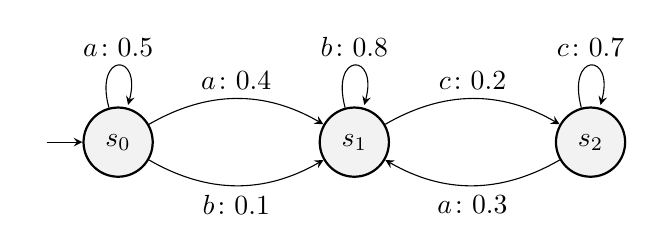
\begin{tikzpicture}
            \tikzset{
                ->, % usmerjene povezave
                >=stealth, % izražitejša konica puščice
                node distance=3cm, % minimalna razdalja med stanjema
                every state/.style={thick, fill=gray!10}, % sets the properties for each ’state’ node
                initial text=$ $, % vhodna puščica v začetno stanje
            }

            \node[state, initial] (s0) {$s_0$};
            \node[state, right of=s0] (s1) {$s_1$};
            \node[state, right of=s1] (s2) {$s_2$};

            \draw 
            (s0) edge[loop above] node{$a \colon 0.5$} (s0)
            (s0) edge[bend left, above] node{$a \colon 0.4$} (s1)
            (s0) edge[bend right, below] node{$b \colon 0.1$} (s1)
            (s1) edge[loop above] node{$b \colon 0.8$} (s1)
            (s1) edge[bend left, above] node{$c \colon 0.2$} (s2)
            (s2) edge[loop above] node{$c \colon 0.7$} (s2)
            (s2) edge[bend left, below] node{$a \colon 0.3$} (s1);
        \end{tikzpicture}
        \caption{Shema končnega vira}
        \label{fig:FSM}
    \end{figure}
    Določimo verjetnost, da naš informacijski vir generira nize $\mathit{cba}$, $\mathit{abcab}$, 
    $\mathit{aabcabc}$. Vedno začnemo v začetnem stanju $s_0$. Ker iz se iz začetnega stanja 
    ne ne moremo premakniti v nobeno drugo stanje s črko $s$, je
    \[
        \mu(\mathit{cba}) = 0.
    \]
    Niz $\mathit{acca}$ lahko generiramo samo z enim zaporedjem vozlišč 
    $s_0$, $s_1$, $s_2$, $s_2$, $s_1$, zato je
    \begin{align*}
        \mu(\mathit{acca}) &= p(a, s_1|s_0)p(c, s_2|s_1)p(c, s_2|s_2)p(a, s_1|s_2) \\
        &= 0.4 \cdot 0.2 \cdot 0.7 \cdot 0.3 \\
        &\approx 0.0168.
    \end{align*}
    Niz $\mathit{abc}$ lahko generiramo z zaporedjem $s_0, s_0, s_1, s_2$ ali pa s
    $s_0, s_1, s_1, s_2$, zato je
    \begin{align*}
        \mu(\mathit{abc}) &= p(a, s_0|s_0)p(b, s_1|s_0)p(c, s_2|s_1) 
        + p(a, s_1|s_0)p(b, s_1|s_1)p(c, s_2|s_1) \\
        &= 0.5 \cdot 0.1 \cdot 0.2 + 0.4 \cdot 0.8 \cdot 0.2 \\
        &\approx 0.74.
    \end{align*}
\end{primer}

\begin{opomba} %finite state automata
    Končni viri abecede $\A$ stopnje $m$ so tesno povezani s končnimi avtomati.
\end{opomba}

Več o odvečnost, kot smo jo definirali, v povezavi s končnih virov abecede $\A$ stopnje $m$,
najdemo v~\cite{Plotkin1992}.

\section{Kontekstno-neodvisne gramatike}

Pravopis določa pravila o rabi črk in ločil. Slovnica je sistem pravil 
za tvorjenje povedi in sestavljanje besedil. Slovenska slovnica, Slovenski pravopis in Slovar 
slovenskega knjižnega jezika določajo slovenski knjižni jezik, ki je poglavitno sredstvo javnega 
in uradnega sporazumevanja v Sloveniji. Podobno je \emph{formalna gramatika} sistem pravil, ki pove
kako iz dane abecede tvorimo nize oziroma kateri nizi so ``pravilni''. Veljavne nize imenujemo 
\emph{formalni jezik}. Formalne gramatike in formalni jeziki imajo široko uporabo. Uporabljajo se
za modeliranje naravnih jezikov, kompresijo podatkov, so osnova programskih jezikov ter 
formalizirajo matematično logiko in sisteme aksiomov.

Definicijo formalne gramatike poda Chomsky v~\cite{Chomsky1956} in jih razdeli v štiri razrede z 
postopnim povečevanjem omejitev~\cite{Chomsky1959, ChomskySchutzenberger1963}.
V delu bomo spoznali le en razred formalnih gramatik, in sicer \emph{Kontekstno-neodvisne gramatike}.

\begin{definicija}
    Relacija $ P \subseteq A \times B $ je \emph{celovita}, če velja 
    $\forall x \in A \ \exists y \in B \colon (x,y) \in P$.
\end{definicija}

\begin{definicija}
    \emph{Kontekstno-neodvisna gramatika}, je četverica $G = (V, \Sigma, P, S)$,
    kjer je
    \begin{itemize}
        \item $V$ abeceda \emph{nekončnih simbolov};
        \item $\Sigma$ abeceda \emph{končnih simbolov} taka, da $\Sigma \cap V = \emptyset$;
        \item $P \subseteq V \times ( V \cup \Sigma )^*$ celovita relacija, elementom 
        relacije pravimo \emph{prepisovalna pravila};
        \item $S \in V$ je \emph{začetni simbol}.
    \end{itemize}
\end{definicija}

\begin{definicija}
    Naj bo $G$ kontekstno-neodvisna gramatika in $\alpha$, $\beta$, $\gamma \in (V \cup \Sigma)^*$,
    $A \in V$ ter naj bo $(A, \beta) \in P$, pišemo $A \rightarrow \beta$. 
    \emph{Levi član prepisovalnega pravila $A \rightarrow \beta$} je $A$ in 
    \emph{desni član prepisovalnega pravila} je $\beta$. Pravimo, da se 
    $\alpha A \gamma$ \emph{prepiše s pravilom} $A \rightarrow \beta$ v $\alpha\beta\gamma$,
    pišemo $\alpha A \gamma \Rightarrow \alpha\beta\gamma$. Pravimo, da $\alpha $ \emph{izpelje} 
    $\beta$, če je $\alpha = \beta$ ali če za $k \geq 0$ obstaja zaporedje 
    $\alpha_1, \alpha_2, \ldots, \alpha_n \in (V \cup \Sigma)^+$, da 
    \[
        \alpha = \alpha_1 \Rightarrow \alpha_2 \Rightarrow \ldots \Rightarrow \alpha_n
        = \beta,
    \]
    kar krajše pišemo $\alpha \xRightarrow{*} \beta$. Kontekstno-neodvisno gramatiko okrajšamo s KNG.
\end{definicija}

\begin{primer}
    Naj bo $ V = \{ S\}$, 
    $\Sigma = \{ a,b \}$, 
    $P = \{ S \rightarrow aSb, S \rightarrow \epsilon \}$ in
    $S = S$.
    To je res KNG, saj sta množici $V$ in $\Sigma$ končni in disjunktni ter je $P$ celovita.
    Izpeljemo nize
    \begin{gather*}
        S \Rightarrow \epsilon, \\
        S \Rightarrow \mathit{aSb} \Rightarrow \mathit{ab}, \\
        S \Rightarrow \mathit{aSb} \Rightarrow \mathit{aaSbb} \Rightarrow \mathit{aabb}, \\
        \vdots
    \end{gather*}
\end{primer}

Ime kontekstno-neodvisna gramatika izvira iz oblike prepisovalnih pravil. Na levi strani 
pravila mora vedno stati samo en nekončni simbol. Torej, ne sme vsebovati pravil oblike 
$\alpha A \gamma \rightarrow \alpha\beta\gamma$, saj je uporaba tega pravila odvisna od 
\emph{konteksta} nekončnega simbola $A$. Kontekst določa niza 
$\alpha, \beta \in ( V \cup \Sigma )^*$, ki se nahajata neposredno pred in po nekončnim simbolom.

Standardno z velikimi tiskanimi črkami označujemo nekončne simbole, z malimi tiskanimi črkami 
označujemo končne simbole in z grškimi črkami označujemo končne nize nekončnih in končnih simbolov.
Ko govorimo o poljubnem simbolu, ga označimo z $y$.

\begin{definicija}\label{primer:kng}
    Jezik KNG $G$ je $L(G) = \{ w \in \Sigma^* \mid S \xRightarrow{*} w \}$. Jezik so torej nizi,
    ki jih lahko izpelejmo s pravili iz začetnega simbola in vsebujejo le končne simbole.
\end{definicija}

\begin{primer}
    Jezik KNG iz primera~\ref{primer:kng} je $\{ a^n b^n \mid n \geq 0 \}$.
\end{primer}

\begin{primer}
    Formalizirajmo formalno gramatiko iz primera~\ref{primer:motivacija}. Pridelali smo jo z nizom
    $w = \mathit{cababcccababcccab} $. Označimo jo z $ G_w = (V, \Sigma, P, S) $, kjer je 
    \begin{gather*}
        V = \{ S, A, B, C \}, \\
        \Sigma = \{ a, b, c \}, \\
        P = \{ S \rightarrow \mathit{cCCA}, A \rightarrow \mathit{ab}, B 
        \rightarrow \mathit{ccc}, C \rightarrow \mathit{AAB} \}, \\
        S = S.
    \end{gather*}
    Vidimo, da je $G_w$ KNG in $ L(G_w) = \{w\} $.
\end{primer}

\subsection{Dopustne gramatike}

Da lahko stistnemo niz $w$ s pomočjo KNG mora biti njen jezik enojec $\{ w \}$, saj lahko
iz KNG enolično rekonstruramo niz $w$. V razdelku predstavimo poseben primer KNG, to so
\emph{dopustne gramatike}~\cite{KiefferYang2000}.

\begin{definicija}
    KNG $G$ je \emph{deterministična}, če vsak nekončen simbol $ A \in V $, nastopa natanko enkrat
    kot levi član nekega prepisovalnega pravila. KNG, ki ni deterministična, je 
    \emph{nedeterministična}.
\end{definicija}

Determinističnost zagotovi, da je prepisovalno pravilo natanko določeno z njegovim levim članom.
Ko se odločimo, da bomo uporabili pravilo katerega levi član je $A$, je takšno pravilo natanko eno. 

\begin{trditev}\label{trditev:DetJezik}
    Naj bo $G$ deterministična KNG. Potem je jezik $G$ enojec ali pa prazna množica.
\end{trditev}

\begin{dokaz}
    Recimo, da je $L(G) \neq \emptyset$ in da vsebuje več kot en niz. Naj bosta $w, u \in L(G)$
    in $w \neq u$. Potem obstajata različni izpeljavi $S \xRightarrow{*} w$ in 
    $S \xRightarrow{*} u$. Ker sta različni, smo v zaporedju izpeljave izbirali med dvema 
    različnima prepisovalnima praviloma. To je v protislovju z determinističnostjo. Torej je 
    $w = u$ in obstaja le ena izpeljava niza iz $S$.
\end{dokaz}

Determinizem sam po sebi ni dovolj močan, da prepreči praznost jezika, kot nam pokažeta sledeča
primera, kjer se v izpeljavi ``zaciklamo''. Zato bomo od dopustnih gramatik zahtevali, da je 
njihov jezik neprazen.

\begin{primer}
    Naj bo $G$ KNG in $V = \{ S \}$, $\Sigma = \{ a \}$, $P = \{ S \rightarrow S \}$, $S = S$.
    KNG je deterministična. Jezik je prazen, saj ne moremo izpeljati niza, ki bi vseboval le
    končne simbole.
\end{primer}

\begin{primer}
    Naj bo G KNG in $V = \{ S, A, B \} $, $\Sigma = \{ a \}$, 
    $P = \{ S \rightarrow \mathit{Aa}, A \rightarrow \mathit{Ba}, B \rightarrow Aa \}$, $S = S$. 
    KNG je deterministična. Jezik je prazen, saj ne moremo izpeljati niza, ki bi vseboval le 
    končne simbole. Z uporabo končno mnogo prepisovalnih pravil se le ciklamo med $A$ in $B$, 
    pri tem nam število ponovitev končnega simbola $a$ pove kolikokrat smo uporabili pravila.
    \[
        S \Rightarrow \mathit{Aa} \Rightarrow \mathit{Baa} \Rightarrow \mathit{Aaaa} \Rightarrow
        \mathit{Baaa} \Rightarrow\ldots
    \]
\end{primer}

Ker bomo KNG stisnili, da ne vsebuje odvečnih simbolov. Simbol ni odvečen, če se pojavi v vsaj 
eni izpeljavi niza, ki je v jeziku. 

\begin{definicija}
    Pravimo, da KNG $G$ \emph{ne vsebuje neuporabnih simbolov}, 
    ko za vsak simbol $ y \in V \cup \Sigma, \ y \neq S $, obstajajo nizi
    $ \alpha_1, \alpha_2, \ldots, \alpha_n \in (V \cup \Sigma)^+ $ tako, da je $y$ vsebovan vsaj
    v enem izmed nizov in velja
    \[
        S \Rightarrow \alpha_1 \Rightarrow \alpha_2 \Rightarrow \cdots \Rightarrow \alpha_n \in L(G).
    \]
\end{definicija}

Zgornje zahteve sedaj združimo v nov podrazred KNG. 
% Ljupčo - zakaj intuitivno zahtevamo odsotnosti praznega niza?

\begin{definicija}
    KNG $G$ je \emph{dopustna gramatika}, če je deterministična, ne vsebuje neuporabnih simbolov,
    $ L(G) \neq \emptyset $ in prazen niz ne nastopa kot desni član kateregakoli prepisovalnega 
    pravila v $ P $.
\end{definicija}

\begin{posledica}
    Jezik dopustne gramatike je enojec. 
\end{posledica}

\begin{dokaz}
    Direktno sledi iz trditve~\ref{trditev:DetJezik} in zahteve po nepraznosti jezika dopustne 
    gramatike.
\end{dokaz}

Če je $G$ dopustna gramatika, obstaja enolično določen $w \in \Sigma(G)^+$, da je
$L(G) = \{ w \}$. Zato jo bomo pogosto označili kar z $G_w$ in rekli, da generira niz $w$.

Prepisovalna pravila točno določajo KNG, saj lahko iz njih enolično določimo $V$, $\Sigma$ in $S$.
Nekončni simboli so levi člani prepisovalnih pravil, končni simboli so desni člani prepisovalnih
pravil, ki niso tudi levi člani kateregakoli prepisovalnega pravila in začetni simbol je nekončni
simbol, ki ne nastopa kot desni član kateregakoli prepisovalnega pravila. Torej je dovolj, da 
stisnemo le prepisovalna pravila.

\begin{primer}\label{primer:dopustna}
    Podana so prepisovalna pravila
    \[
        P = \{ A \rightarrow \mathit{aBCD}, B \rightarrow \mathit{ab}, C \rightarrow 
        \mathit{Bb}, D \rightarrow \mathit{Cb} \}.
    \]
    Sledimo zgornjemu razmisleku in dobimo, da je $V = \{ A, B, C, D \}$, $\Sigma = \{ a, b \}$.
    $S = A$. Vidimo, da je $L(G) = \mathit{aababbabbb}$ Zlahka preverimo, da je KNG. Da je dopustna,
    bomo preverili kasneje.
\end{primer}

\subsection{D0L-sistem}

Kot nas je pri uvedbi formalne gramatike motivirala slovnica, nas sedaj motivira biologija.
Procese, ki potekajo istočaso, na primer razmnoževanja bakterij ali rast rastlin, lahko opišemo z
\emph{Lindenmayerjevim sistemom}, krajše \emph{$L$-sistemom}. Ker se ukvarjamo z dopustnimi
gramatikami, se omejimo na \emph{deterministične kontekstno-neodvisne $L$-sisteme}. Več o splošnih
$L$-sistemih najdemo v~\cite{RozenbergSalomaa2012}.

\begin{definicija}
    Naj bo $\Sigma$ abeceda. \emph{Endomorfizem na $\Sigma^*$} je preslikava 
    $f \colon \Sigma^* \to \Sigma^* $ tako, da je
    \begin{gather*}
        f(\varepsilon) = \varepsilon, \\
        \forall w, u \in \Sigma^* \colon f(wu) = f(w)f(u).
    \end{gather*}
    Induktivno definiramo
    \begin{align*}
        f^0(w) &= w, \\
        f^1(w) &= f(w), \\
        f^k(w) &= f(f^{k-1}(w)),
    \end{align*}
    kjer je $w \in \Sigma^*$ in $k \geq 2$ celo število.
\end{definicija}

\begin{opomba}
    Endomorfizem $f$ na $\Sigma^*$ je natanko določen, ko za vsako črko $a \in \Sigma$ podamo 
    njeno preslikavo $f(a) \in \Sigma^*$.
\end{opomba}

\begin{definicija}
    \emph{Deterministični kontekstno-neodvisni $L$-sistem}, na kratko \emph{D0L-sistem},
    je trojica $D = (\Sigma, f, w)$, kjer je $\Sigma$ abeceda; $f$ endomorfizem na $\Sigma^*$;
    in $w \in \Sigma^*$. Sistem ima \emph{fiksno točko $ w^* $}, če za zaporedje 
    $\{ f^k(w) \mid k = 0, 1,2 \ldots \}$ velja
    \begin{gather*}
        w^* \in \{ f^k(w) \mid k = 0, 1, 2, \ldots \}, \\
        f(w^*)= w^*.
    \end{gather*}
\end{definicija}

\begin{definicija}
    Naj bo $G$ deterministična KNG v kateri prazen niz ne nastopa kot desni član kateregakoli 
    prepisovalnega pravila. Na $(V \cup \Sigma)^*$ definiramo endomorfizem $f_G$ tako, da
    \begin{gather*}
        \forall a \in \Sigma \colon f_G(a) = a; \\
        \text{če je } A \rightarrow \alpha \text{ prepisovalno pravilo, potem je } f_G(A) = \alpha.
    \end{gather*}
    D$0$L-sistem $(V \cup \Sigma, f_G, S)$ označimo z D$0$L$(G)$ in ga imenujemo 
    \emph{D0L-sistem prirejen $G$}.
\end{definicija}

Če uporabimo $f_G$ na nekem nizu nekončnih in končnih simbolov, uporabimo v enem koraku vsa 
prepisovalna pravila, ki jih lahko. Medtem, ko pri KNG v vsaki 
iteraciji uporabimo le eno prepisovalno pravilo naenkrat.

\begin{primer}\label{primer:fiksna}
    Spomnimo se KNG $G$ iz primera~\ref{primer:dopustna} in ji priredimo D$0$L-sistem. Prepisovalna
    pravila so
    \[
        P = \{ A \rightarrow \mathit{aBCD}, B \rightarrow \mathit{ab}, C \rightarrow 
        \mathit{Bb}, D \rightarrow \mathit{Cb} \}.
    \] 
    Ker je $G$ deterministična in prazni niz ne nastopa kot desni član kateregakoli prepisovalnega
    pravila, ji lahko priredimo D$0$L$(G)$. Potem je $S = A$, $f_G(a) = a$, $f_G(b) = b$ in 
    $f_G(A) = aBCD$, $f_G(B) = ab$, $f_G(C) = Bb$, $f_G(D) = Cb$. Izračunajmo še fiksno točko:
    \begin{align*}
        f_G^0(A) &= A, \\
        f_G^1(A) &= \mathit{aBCD}, \\
        f^2_G(A) &= \mathit{aabBbCb}, \\
        f^3_G(A) &= \mathit{aababbBbb}, \\
        f^4_G(A) &= \mathit{aababbabbb}.
    \end{align*}
    Vidimo, da je fiksna točka enaka nizu, ki ga izpelje $G$.
\end{primer}

\begin{trditev}\label{trditev:fiksna}
    Naj bo $G$ dopustna gramatika. Potem je $ w \in L(G)$ fiksna točka D0L$(G)$.
\end{trditev}

\begin{dokaz}
    Ker je $G$ dopustna, je deterministična in prazen niz ne nastopa kot desni član kateregakoli
    prepisovalnega pravila. Torej ji lahko priredimo D$0$L$(G)$. Prav tako velja, da je jezik 
    enojec, torej $L(G) = \{ w \}$.
    
    Imamo prepisovalno pravilo $S \rightarrow \alpha$, kjer je $\alpha \in (V \cup \Sigma)^*$.
    Naj bo $y_1 y_2 \cdots y_n$ predstavitev niza $\alpha$ s črkami. Potem je
    \[
        f^i_G(S) = f^i_G(y_1 y_2 \cdots y_n) = f^i_G(y_1)f^i_G(y_2) \cdots f^i_G(y_n).
    \]
    Če je $y_j \in \Sigma$, potem je $f^i_G(y_j) = y_j$, sicer pa $y_j \in V$ in zaradi 
    determinističnosti obstaja prepisovalno pravilo $y_j \rightarrow z$, kjer je 
    $z \in (V \cup \Sigma)^*$. Torej je $f^i_G(y_i) = f^{i-1}_G(z)$. 
    
    Ker so množice $V$, $\Sigma$, $P$ končne in $S$ izpelje $w$, obstaja tak $i \in N$, da je 
    $f^i_G(S) = w$. Niz $ w \in \Sigma^+ $ je res fiksna točka, saj je 
    \[
        f_G(w) = f_G(w_1w_2 \cdots w_n) = f_G(w_1)f_G(w_2) \cdots f_G(w_n) = w_1w_2 \cdots w_n = w,
    \]
    kjer so $w_1, w_2, \ldots, w_n \in \Sigma$.
\end{dokaz}

\subsection{Izpeljevalni graf}

\begin{definicija}
    Naj bo $G$ KNG v kateri prazen niz ne nastopa kot desni član kateregakoli
    prepisovalnega pravila. \emph{Izpeljevalni graf $G$}, označimo ga z $\Gamma(G)$, je 
    usmerjen graf z vozlišči $ V \cup \Sigma $. Za prepisovalno pravilo
    \[    
        A \rightarrow y_1 y_2 \cdots y_n,
    \]
    iz vozlišča $A$ izvirajo usmerjene povezave v vozlišča $y_1, y_2, \ldots, y_n \in V \cup \Sigma$.
\end{definicija}

Osvežimo osnovni definiciji iz teorije grafov.

\begin{definicija}
    % To kar definiram kot pot je načeloma sprehod, za pot bi morali zahtevati še, da so vozlišča paroma različna
    % Vendar vemo, da če obstaja sprehod od u do v, potem obstaja tudi pot od u do v
    \emph{Pot dolžine $n$} je zaporedje vozlišč $(v_1, v_2, \ldots, v_{n+1})$, da za vsak 
    $i = 1, 2, \ldots, n$ velja, da je $(v_i,v_{i+1})$ povezava v grafu. 
    Pravimo, da je pot \emph{cikel}, če je $v_1 = v_{i+1}$. Graf brez ciklov je \emph{acikličen}.
\end{definicija}

\begin{definicija}
    Vozlišče $v$ je \emph{koren usmerjenega grafa}, če je za vsako vozlišče $u \neq v$ obstaja
    pot od $v$ do $u$.
\end{definicija}

\begin{primer}\label{primer:izpeljevalni}
    Poglejmo izpeljevalni graf KNG $G$ iz primera~\ref{primer:dopustna}. Prepisovalna pravila so
    \[
        P = \{ A \rightarrow \mathit{aBCD}, B \rightarrow \mathit{ab}, C \rightarrow 
        \mathit{Bb}, 
        D \rightarrow \mathit{Cb} \}.
    \]
    \begin{figure}[H]
        \centering
        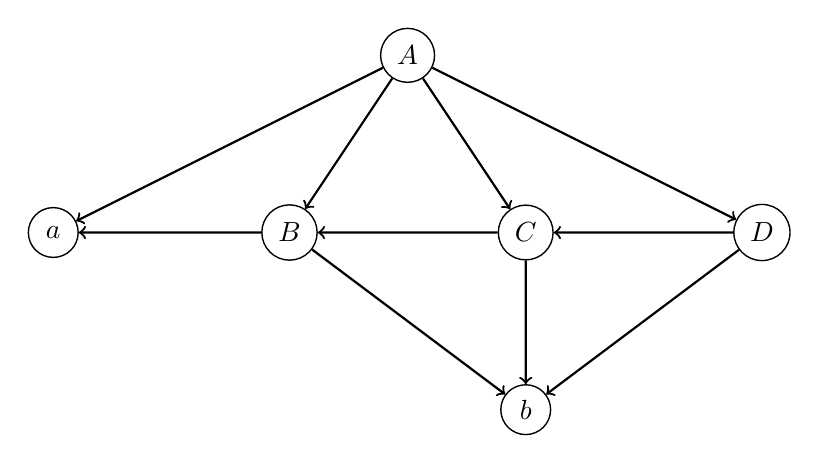
\begin{tikzpicture}[scale=1.5]
            \GraphInit[vstyle=Normal]
            \SetUpEdge[style={->}] % Usmerjen graf
            
            \Vertex[Lpos=270,L=$A$,x=0,y=0]{A}
            \Vertex[Lpos=270,L=$a$,x=-3,y=-1.5]{a} 
            \Vertex[Lpos=270,L=$B$,x=-1,y=-1.5]{B}
            \Vertex[Lpos=270,L=$C$,x=1,y=-1.5]{C}
            \Vertex[Lpos=270,L=$D$,x=3,y=-1.5]{D}
            \Vertex[Lpos=270,L=$b$,x=1,y=-3]{b}
            
            \Edge (A)(B)
            \Edge (A)(a)
            \Edge (A)(C)
            \Edge (A)(D)
            \Edge (B)(a)
            \Edge (C)(B)
            \Edge (D)(C)
            \Edge (B)(b)
            \Edge (C)(b)
            \Edge (D)(b)
        \end{tikzpicture}
    \caption{Izpeljevalni graf $\Gamma(G)$.}
    \end{figure}
\end{primer}

\begin{lema}\label{lema:koren}
    Naj bo $G$ dopustna gramatika. Potem ima $\Gamma(G)$ koren $S$.
\end{lema}

\begin{dokaz}
    Naj bo $y \in V \cup \Sigma$ različno od $S$. Poiščemo pot od $S$ do $y$. Ker je $G$ dopustna,
    ne vsebuje neuporabnih simbolov. Po definiciji za $y \in V \cup \Sigma$, $ y \neq S$, obstajajo
    $\alpha_1, \alpha_2, \ldots, \alpha_n \in (V \cup \Sigma)^+$, da je $y$ vsebovan vsaj
    v enem izmed njih in velja $S \Rightarrow \alpha_1 \Rightarrow \alpha_2 \Rightarrow \cdots 
    \Rightarrow \alpha_n \in L(G)$.
    
    Recimo, da $y$ prvič nastopi v $\alpha_k$. Velja, da 
    \begin{gather*}
        y \text{ nastopa v } \alpha_k; \\
        S \rightarrow \alpha_1; \\
        \text{če je } k > 1 \text{, potem } \forall i = 1, 2, \ldots, k-1 \colon \alpha_i 
        \Rightarrow \alpha_{i+1}.
    \end{gather*}
    Zgradimo pot z indukcijo na $k$. Za $k=1$, je $y$ vsebovan v $\alpha_1$, torej je pot kar 
    povezava med $S$ in $y$. Naj bo sedaj $k>1$ in predposatvimo, da obstaja pot od $S$ do vsakega
    simbola v $\alpha_{k-1}$. Izberemo tisti $A \in V$, ki iz $\alpha_{k-1}$ izpelje $\alpha_k$.
    Ker $y$ nastopa v $\alpha_k$, obstaja povezava med $A$ in $y$. Po predpostavki obstaja pot
    med $S$ in $A$, zato $A$ nastopa v $\alpha_{k-1}$. Našli smo pot od $S$ do $y$.
\end{dokaz}

\begin{lema}\label{lema:acikličen}
    Naj bo $G$ dopustna gramatika. Potem je $\Gamma(G)$ acikličen.
\end{lema}

\begin{dokaz}
    Po trditevi~\ref{trditev:fiksna} obstaja fiksna točka $w$ endomorfizma $f_G$. Torej, obstaja
    $i = 1, 2, \ldots$, da je $f^i_G(w) = w \in \Sigma^+$. To pomeni, da 
    \begin{gather}\label{gather:acikel}
        \text{končno mnogo členov zaporedja } \{ f^i_G(S) \mid i = 1, 2, \ldots \} \text{ ni niz v }
        \Sigma^+.
    \end{gather}
    
    Naj bosta $A, B \in V$ med katerima obstaja pot od $A$ do $B$. Ker je $G$ dopustna, ne vsebuje
    neuporabnih simbolov. Za $A$ obstajajo $\alpha_1, \alpha_2, \ldots, \alpha_n \in (V \cup \Sigma)^+$ 
    tako, da $A$ nastopa v vvsaj v enem izmed njih in $S \Rightarrow \alpha_1 \Rightarrow 
    \alpha_2 \Rightarrow \cdots \Rightarrow \alpha_n \in L(G)$. To pomeni, da $A$ nastopa v
    $f^i_G(S)$ za nek $i = 1, 2, \ldots$. Ker obstaja pot od $A$ do $B$, potem $B$ nastopa v 
    nekem $f^j_G(S)$ za nek $j = i+1, i+2, \ldots$.

    Recimo da ima grafu $\Gamma(G)$ cikel. Torej, obstaja neka pot od $A$ do $A$. Potem se $A$
    pojavi neskončnokrat v zaporedju $\{ f^i_G(S) \mid i = 1, 2, \ldots \}$, to pa je v 
    protislovju z izjavo~\ref{gather:acikel}, ki sledi iz predpostavke.
\end{dokaz}

\subsection{Karakterizacija dopustne gramatike}

Preko izpeljevalnega grafa gramatike lahko ugotovimo ali je podana gramatika dopustna. Tudi preko
D$0$L-sistema gramatike lahko preizkusimo dopustnost gramatike. Še več, D$0$L-sistem gramatike
nam poda algoritem za izračun niza, ki ga generira dopustna gramatika.

\begin{izrek}\label{izrek:ekvivalence}
    Naj bo $G$ KNG v kateri prazen niz ne nastopa kot desni član 
    kateregakoli prepisovalnega pravila. Potem so naslednje trditve ekvivalentne:
    \begin{enumerate}
        \item $G$ je dopustna gramatika.
        \item $\Gamma(G)$ je acikličen in ima koren $S$.
        \item Za D0L$(G)$ je $ f_G^{\abs{V}}(S) \in \Sigma^+ $ in vsak simbol iz
        $ V \cup \Sigma $ nastopa v vsaj enem izmed nizov $f_G^i(S)$ za $i=0, 1, \ldots, \abs{V}$.
    \end{enumerate}
\end{izrek}

Pred dokazom zgornjega izreka potrebujemo še tri leme, ki bodo pomagale pri dokazu.

\begin{lema}\label{lema:pomožna}
    Naj bo $G$ KNG v kateri prazen niz ne nastopa kot desni član kateregakoli prepisovalnega 
    pravila in $\Gamma(G)$ acikličen. Vzemimo $\alpha \in ( V \cup \Sigma)^+ \setminus \Sigma^+$.
    Potem obstaja nekončni simbol $ A \in V $, ki nastopa v nizu $\alpha$ in za $\forall i=1,2,\ldots$
    velja
    \[
        A \text{ ne nastopa v nizu } f^i_G(\alpha).
    \]
\end{lema}

\begin{dokaz}
    Dokažimo s protislovjem. Predpostavimo, da zaključek leme ne velja. Z $H$ označimo vse 
    nekončne simbole $V$, ki nastopajo v $\alpha$. Po predpostavki je $H$ neprazna. Za vsak 
    $B \in H$ definiramo 
    \[
        H(B) = \{ C \in V \mid C \text{ nastopa v enem izmed nizov } f^i_G(B), \ i= 1, 2, \ldots \}.
    \]
    Vsak nekončen simbol iz $V$, ki nastopa v enem izmed $f^i_G(\alpha)$, kjer je $i= 1, 2, \ldots$,
    leži v $\cup_{B \in H}H(B)$. Po predpostavki
    \[
        \forall A \in V \colon A \notin H \vee A \text{ nastopa v enem izmed nizov } f^i_G(\alpha),
        \ i= 1, 2, \ldots
    \]
    sledi, da za vsak $A \in H$ obstaja $B \in H$ tako, da je $A \in H(B)$.

    Sedaj izberemo takšno neskončno zaporedje $A_1, A_2, \ldots$ elementov $H$, da za vsak
    $i= 1, 2, \ldots$ velja $A_i \in H(A_{i+1})$. Ker je množica $H$ končna, obstaja nek 
    $A$ in naravni števili $i < j$, da je $A_{i} = A_{j} = A$.

    Opomnimo, da za $A \in H(B)$, obstaja pot od $B$ do $A$ v grafu $\Gamma(G)$. 
    Torej, v zaporedju $A_1, A_2, \ldots$, obstaja pot
    \[
        (A_j, A_{j-1}, \ldots, A_{i+1}, A_i).
    \]
    Ker je ta pot cikel smo prišli do protisolovja.
\end{dokaz}

\begin{lema}\label{lema:izračun}
    Naj bo $G$ KNG v kateri prazen niz ne nastopa kot desni član 
    kateregakoli prepisovalnega pravila in $\Gamma(G)$ acikličen. Potem je
    \[
        \forall \alpha \in ( V \cup \Sigma)^+ \colon f^{\abs{V}}_G(\alpha) \in \Sigma^+.
    \]
\end{lema}

\begin{dokaz}
    Naj bo $ \alpha \in ( V \cup \Sigma)^+ $ poljuben. Predpostavimo, da 
    $ f^{\abs{V} }_G(\alpha) \notin \Sigma^+ $ in pokažimo, da nas to vodi v
    protislovje.

    Po predpostavki in ker je $\forall a \in \Sigma$ velja $f_G(a) = a$, sklepamo, da niz 
    $f^i_G(\alpha)$, kjer je $i= 0, 1, \ldots, \abs{V}$, vsebuje vsaj en nekončen simbol iz $V$. 
    Na vsakem nizu $f^i_G(\alpha)$ uporabimo lemo~\ref{lema:pomožna} in dobimo zaporedje 
    $A_0, A_1, \ldots, A_{\abs{V}}$ nekončnih simbolov iz $V$, da za $i= 0, 1, \ldots, \abs{V}$ 
    velja
    \begin{gather}
            A_i \text{ nastopa v nizu } f^i_G(\alpha); \label{gather:nastopa} \\
            \forall j = i+1, i+2, \ldots, \abs{V} \colon A_i \text{ 
            ne nastopa v nizu } f^j_G(\alpha). \label{gather:nenastopa}
    \end{gather}
    
    Ker je zaporedje $A_0, A_1, \ldots, A_{\abs{V}}$ simbolov iz $V$, daljše od $\abs{V}$, se vsaj
    en simbol ponovi. Torej, obstaja $A \in V$ in $i,j \in \{0, 1, \ldots, \abs{V} \}$, $i<j$, 
    da je $A_i = A_j = A$.

    Po~\ref{gather:nastopa} $A_i$ nastopa v $f^i_G(\alpha)$ ter po~\ref{gather:nenastopa} ne 
    nastopa v $f^j_G(\alpha)$. Vendar po~\ref{gather:nastopa} tudi $A_j$ nastopa v $f^j_G(\alpha)$.
    Ker je $A_i = A_j = A$, smo prišli do protislovja.
\end{dokaz}

\begin{lema}\label{lema:nastopanje}
    Naj bo $G$ KNG v kateri prazen niz ne nastopa kot desni član 
    kateregakoli prepisovalnega pravila in naj bo $\Gamma(G)$ acikličen ter ima
    koren $S$. Potem vsak simbol iz $V \cup \Sigma$ nastopi v vsaj enem izmed nizov $f^i_G(S)$, 
    $i= 0, 1, \ldots, \abs{V}$. 
\end{lema}

\begin{dokaz}
    Če v grafu $\Gamma(G)$ obstaja pot dolžine $i$ od $A \in V$ do $y \in V \cup \Sigma$, potem
    simbol $y$ nastopa v $f^i_G(A)$. Koren $S$ očitno nastopa v nizu $f^0_G(S)$. Izberemo poljuben
    $y \in V \cup \Sigma$ različen od $S$. Ker je $S$ koren grafa, obstaja pot dolžine 
    $i$ od $S$ do $y$. 
     
    Pot je oblike $(S, A_2, A_3, \ldots, A_i, y)$, kjer so $S, A_2, A_3, \ldots, A_i \in V$. Ker 
    je graf brez ciklov, so vsa vozlišča $S, A_2, A_3, \ldots, A_i$ paroma različna. Res je 
    $i < \abs{V}$.
\end{dokaz}

Sedaj lahko dokažemo izrek. 

\begin{dokaz}[Dokaz izreka~\ref{izrek:ekvivalence}]
    \mbox{}
    \begin{itemize}
        \item[$1\Rightarrow 2$] Sledi po lemah~\ref{lema:koren} in~\ref{lema:acikličen}.
        \item[$2\Rightarrow 3$] Sledi po lemah~\ref{lema:izračun} in~\ref{lema:nastopanje}.
        \item[$3\Rightarrow 1$] Obstoj D$0$L$(G)$ nam zagotovi determinističnost in da
        prazen niz ne nastopa kot desni član kateregakoli prepisovalnega pravila. 
        
        Jezik je neprazen, saj $f_G^{\abs{V}}(S) \in \Sigma^+$. 

        Ne vsebuje neuporabnih simbolov, saj vsak simbol iz $V \cup \Sigma$ nastopa v vsaj enem 
        izmed nizov $f_G^i(S)$, kjer je $i=0, 1, \ldots, \abs{V}$.
    \end{itemize}
\end{dokaz}

\begin{primer}
    Preverimo dopustnost gramatike iz primer~\ref{primer:dopustna}. 
    V primeru~\ref{primer:izpeljevalni} smo narisali izpeljevalni graf te gramatike. Ker je graf
    acikličen in koren $S$, je gramatika dopustna po $2.$ točki izreka~\ref{izrek:ekvivalence}.
    V primeru~\ref{primer:fiksna} smo tej gramatiki priredili D$0$L-sistem. Do niza, ki vsebuje 
    same končne simbole, smo res prišli v $\abs{V} = 4$ iteracijah. Tudi vsak od simbolov
    $A_0, A_1, A_2, A_3, a, b$ se pojavi v izračunanih nizih. Torej je gramatika dopustna po
    $3.$ točki izreka~\ref{izrek:ekvivalence}.
\end{primer}

Kot smo omenili na začetku razdelka, bomo podali algoritem za izračun niza generiranega z dopustno
gramatiko.

\begin{posledica}
    Niz, generiran z $G_w$, je 
    \[
        w = f_G^{\abs{V}}(S).
    \]
\end{posledica}

\begin{dokaz}
    Direktno sledi po $3.$ točki izreka~\ref{izrek:ekvivalence}.
\end{dokaz}

Prav tako posplošimo trditev~\ref{trditev:fiksna}.

\begin{posledica}\label{posledica:razširtev}
    Naj bo $G$ dopustna gramatika in $\alpha \in (V \cup \Sigma)^+$. Potem ima D$0$L sistem
    $(V \cup \Sigma, f_G, \alpha)$ fiksno točko $ w^* \in \Sigma^+$, ki je
    \[
        w^* = f_G^{\abs{V}}(\alpha).
    \]
\end{posledica}

\begin{dokaz}
    Z lemo~\ref{lema:izračun} razširimo $3.$ točko izreka~\ref{izrek:ekvivalence} iz $S$ na 
    vse $\alpha \in (V \cup \Sigma)^+$.
\end{dokaz}

Sledeči endomorfizem nam bo prišel prav v naslednjem poglavju.

\begin{definicija}\label{def:InftyEndo}
    Naj bo $G$ dopustna gramatika. Definiramo preslikavo
    \begin{align*}
        f_G^\infty \colon (V \cup \Sigma)^* &\to (V \cup \Sigma)^*, \\
        \alpha &\mapsto w^*,
    \end{align*}
    kjer je $w^*$ fiksno točko D$0$L-sistema $(V \cup \Sigma, f_G^\infty, \alpha)$.
\end{definicija}

\begin{trditev}
    Naj bo $G$ dopustna gramatika. Potem veljajo naslednje trditve:
    \begin{enumerate}
        \item $f_G^\infty$ je endomorifzem na $(V \cup \Sigma)^*$;
        \item $\forall \alpha \in (V \cup \Sigma)^+ \colon f_G^\infty(\alpha) \in \Sigma^+$ ;
        \item $\forall \alpha \in (V \cup \Sigma)^+ \colon f_G^\infty(\alpha) = f_G^{\abs{V}}(\alpha)$;
        \item Če je $A \rightarrow \alpha$, prepisovalno pravilo, potem je 
        $f_G^\infty(A) = f_G^\infty(\alpha)$.
    \end{enumerate}
\end{trditev}

\begin{dokaz}
    \mbox{}
    \begin{itemize}
        \item[$1.$] Trivialno preverimo, da ustreza definiciji.
        \item [$2.$] Velja po definiciji fiksne točke endomorfizma.
        \item[$3.$] Sledi direktno po~\ref{posledica:razširtev}.
        \item[$4.$] Ker imamo prepisovalno pravilo $A \rightarrow \alpha$ zaporedje e
        $\{ f^k(\alpha) \mid k = 1, 1,2 \ldots \}$ dobimo tako, da odstraimo prvi člen zaporedja
        $\{ f^k(A) \mid k = 0, 1,2 \ldots \}$. Zaporedji imata enako fiksno točko.
    \end{itemize}
\end{dokaz}

\section{Prirejanje in kodiranje dopustne gramatike} 

Vsakemu končnemu nizu $w$ bomo priredili dopustno gramatiko $G_w$, ki generira niz $w$. Dopustni
gramatiki bomo nato priredili binarni niz $B(G_w)$.

\tikzset{block/.style={draw, thick, text width=3cm, minimum height=1.5cm, align=center}, line/.style={-latex}}
\begin{figure}[H]
    \centering
    \scalebox{0.8}{
    \begin{tikzpicture}
        \node (a) {$w$};
        \node[block,right=of a, xshift=6mm] (b) {prirejanje gramatike};
        \node[right=of b, xshift=3mm] (c) {$G_w$};
        \node[block,right=of c, xshift=3mm] (d) {kodiranje gramatike};
        \node[right=of d, xshift=6mm] (e) {$B(G_w)$};

        \draw[line] (a)-- (b);
        \draw[line] (b)-- (c);
        \draw[line] (c)-- (d);
        \draw[line] (d)-- (e);
    \end{tikzpicture}
    }
    \caption{Kodirnik niza $w$}
    \label{fig:Kodirnik}
\end{figure}

Od tu naprej, z $\A$ poljubno abecedo, $\abs{\A} \geq 2$, iz katere bomo tvorili nize. Fiksiramo tudi
končno množico simbolov $\{ A_0, A_1, A_2, \ldots \}$, ki jih bomo uporabljali za nekončne simbole.
Množica $\{ A_0, A_1, A_2, \ldots \}$ ima \emph{naravni abecedni vrstni red} $A_0, A_1, A_2, \ldots$.
Predpostavimo, da je $\A \cap \{ A_0, A_1, A_2, \ldots \} = \emptyset$.

\subsection{Prirejanje gramatike}

Namen dopustne gramatike je generirati niz sestavljen iz simbolov $\A$, zato ni ni pomembno, 
kateri simboli se uporabljajo za nekončne simbole.

\begin{definicija}\label{def:G(A)} 
    Naj bo $\G(\A)$ množica vseh KNG $G$, ki zadostujejo:
    \begin{enumerate}
        \item $G$ je dopustna gramatika;
        \item $\Sigma \subseteq \A$;
        \item $V = \{ A_0, A_1, \ldots, A_{\abs{V}-1} \}$;
        \item $S=A_0$;
        \item Če naštejemo nekončne simbole $V$ v vrstnem redu prve pojavitve od leve proti desni
        v nizu
        \[
            f_G^0(A_0)f_G^1(A_0) \cdots f_G^{\abs{V}-1}(A_0),
        \]
        dobimo zaporedje $A_0, A_1, A_2, \ldots, A_{\abs{V}-1}$.
    \end{enumerate}
    Z lastnostjo $5.$ zahtevamo, da so nekončni simboli poimenovani po edinstvem vrstnem redu To 
    je vrstni red, ki ga inducira iskanje v globino v izpeljevalnem grafu, pri katerem so otroci
    obiskani v vrstnem redu od leve proti desni. Ta razvrstitev bo omogočila dekodirniku v 
    izreku~\ref{izrek:BinarnoKodiranje} določiti ime nove spremenljivke.

KNG $G \notin \G(\A)$, ki izpolnjuje zahtevi $1.$ in $2.$, preimenujmo nekončne simbole tako, da
zadostimo $5.$ točki, Tako pridelamo $[G] \in \G(\A)$ in velja $L([G]) = L(G)$, 
imenujemo jo \emph{kanonično oblika $G$}.
\end{definicija}

\begin{primer}\label{primer:kanonična}
    Naj bo $\A = \{ a,b \}$. Podano imamo dopustno gramatiko $G$ z začetnim simbolov $S$ in 
    prepisovalnimi pravili
    \[
        P = \{ S \rightarrow \mathit{BaC}, A \rightarrow \mathit{aC}, B \rightarrow 
        \mathit{Db}, C \rightarrow \mathit{bB}, D \rightarrow{ab} \}.
    \]
    Zahtevi $1.$ in $2.$ sta izpolnjeni. Izračnajmo $f^i_G(S)$ za $i = 0,1 \ldots, \abs{V-1}$.
    \begin{align*}
        f_G^0(S) &= S, \\
        f_G(S) &= \mathit{BaC}, \\
        f^2_G(S) &= \mathit{DbaaC}, \\
        f^3_G(S) &= \mathit{abbaabB}, \\
        f^4_G(S) &= \mathit{abbaabDb}.
    \end{align*}
    Skupaj staknemo zgornje nize in pridelamo niz iz $5.$ zahteve,
    \[
a        \mathit{SBaCDbaaCabbaabBabbaabDb}.
    \]
    Naštejemo nekončne simbole v vrstnem redu prve pojavitve od leve proti desni v zgornjem nizu:
    $S, B, A, C, D$. 
    
    Glede na ta seznam nekončne simbole ustrezno preimenujemo
    \begin{gather*}
        S \rightsquigarrow A_0, \\
        B \rightsquigarrow A_1, \\
        A \rightsquigarrow A_2, \\
        C \rightsquigarrow A_3, \\
        D \rightsquigarrow A_4.
    \end{gather*}
    Tako pridelamo $[G] \in \G(\A)$ s prepisovalnimi pravili
    \[
        P = \{ A_0 \rightarrow A_1aA_2, A_1 \rightarrow A_3b, A_2 \rightarrow aA_4,
        A_3 \rightarrow ab, A_4 \rightarrow bA_1 \}.
    \]
\end{primer}

Ključni del kodirnika na sliki~\ref{fig:Kodirnik} je prirejanje gramatike. Formalno je prirejanje
preslikava, ki vsakemu nizu abecede $\A$ dodeli gramatiko, ki ta niz generira.

\begin{definicija}
    \emph{Prirejanje gramatike nizu abecede $\A$} je preslikava
    \begin{align*}
        \pi \colon \A^+ &\to \G(\A), \\
        \pi(w) &= G_w.
    \end{align*}
\end{definicija}

Osredotočimo se na dva razreda prirejanj gramatike: asimptotsko kompaktna prirejanje gramatike
in neskrčljivo prirejanje gramatike. Za njuno definicijo bomo potrebovali endoformizem 
iz definicije~\ref{def:InftyEndo}.

\begin{definicija}
    Z $\G^*(\A)$ označimo pravo podmnožico množice $\G(\A)$, da za vsak $G \in \G^*(\A)$ velja
    \[
        \forall A,B \in V, \ A \neq B \colon f_G^\infty(A) \neq f_G^\infty(B).
    \]
\end{definicija}

\begin{definicija}
    Naj bo $G$ dopustna gramatika. Z $\abs{G}$ označimo skupno dolžina desnih članov prepisovalnih
    pravil dopustne gramatike $G$.
\end{definicija}

\subsubsection{Asimptotsko kompaktno prirejanje gramatike}

\begin{definicija}
    Prirejanje gramatike nizu abecede $\A$ je \textit{asimptotsko kompaktna}, če za vsak niz
    $w \in \A^+$ velja $G_w \in \G^*(\A)$ in je
    \[
        \lim_{n \rightarrow \infty} \max_{w \in \A^n} \frac{\abs{G_w}}{\abs{w}} = 0.
    \]
\end{definicija}

Definiramo dve asimptotsko kompaktni prirejanji gramatike, \emph{Lempel-Ziv prirejanje gramatike}
in \emph{bisekcijsko prirejanje gramatike}. Za vsako naredimo tudi primer.

\begin{definicija}
    Naj bo $ w_1w_2 \cdots w_n$ predstavitev niza $w$ z simboli abecede. 
    \emph{Lempel-Ziv členitev niza $w$ abecede $\A$} je množica podnizov $\sigma_\text{lz}(w)$,
    ki jo induktivno gradimo
    \begin{gather*}
        u_1 = w_1 \cdots w_{i_1} \text{ takšen, da ne nastopa v } \sigma_{\text{lz}}(w). \text{ Dodamo }
        u_1 \text{ v } \sigma_{\text{lz}}(w); \\
        u_2 = w_{i_1} \cdots w_{i_2} \text{ takšen, da ne nastopa v } \sigma_{\text{lz}}(w). \text{ Dodamo }
        u_2 \text{ v } \sigma_{\text{lz}}(w); \\
        \vdots \\
        u_{m-1} = w_{i_{m-2}} \cdots w_{i_{m-1}} \text{ takšen, da ne nastopa v } 
        \sigma_{\text{lz}}(w). \text{ Dodamo } u_{m-1} \text{ v } \sigma_{\text{lz}}(w); \\
        u_m = w_{i_{m-1}} \cdots w_n. \text{ Dodamo } u_m \text{ v } \sigma_{\text{lz}}(w).
    \end{gather*}
\end{definicija}

\begin{primer}\label{primer:LZČlenitev}
    Lempel-Ziv členitev niza $w = 010010000001$ je
    \[
    w = \underline{0} \, \underline{1} \, \underline{00} \, \underline{10} \, \underline{000}
    \, \underline{001}.
    \]
    Torej je $\sigma_{\text{lz}}(w) = \{ 0. 1, 00, 10, 000, 001 \}$
\end{primer}

\begin{definicija}[Lempel-Ziv prirejanje gramatike]
    Naj bo $w = w_1w_2 \cdots w_n \in A^+$ in $\sigma_\text{lz}(w) = \{ u_1, u_2, \ldots, u_m \}$.
    Definiramo dopustno gramatiko $G^\text{lz}_w$ tako, da je:
    \begin{itemize}
        \item $\Sigma = \{ u \in \sigma_{\text{lz}}(w) \mid \abs{u} = 1 \}$;
        \item $V = \{ A_w \} \cup \{ A_u \mid u \in \sigma_{\text{lz}}(w) \}$;
        \item $S = A_w$ in imamo prepisovalno pravilo 
        \[ 
            A_w \rightarrow A_{u_1}A_{u_2} \cdots A_{u_m};
        \]
        \item Za $u \in \sigma_{\text{bis}}(w)$ naj bo $u = \alpha b$, kjer je $b \in \Sigma$ in 
        $\alpha \in \Sigma^*$. Za vsak $u \in \sigma_{\text{bis}}(w)$ imamo prepisovalno pravilo
        \[
            A_u \rightarrow A_{\alpha}b.
        \]
    \end{itemize}
    Da dobimo kanonično obliko $[G^\text{lz}_w]$ moramo ustrezno preimenovati nekončne simbole po
    postopku opisanem v deficiji~\ref{def:G(A)} in pokazanem na primeru~\ref{primer:kanonična}.
    Prirejanju $w \mapsto [G^\text{lz}_w]$ pravimo \emph{Lempel-Ziv prirejanje gramatike}.
\end{definicija}

\begin{trditev}
    Lempel-Ziv prirejanje gramatik je asimptotsko kompaktno prirejanje gramatike.
\end{trditev}

\begin{proof}
    Lempel in Ziv sta v~\cite{LempelZiv1976} pokazala, da za velja
    \[
        \max_{w \in \A^n} \abs{\sigma_\text{lz}(w)} = \mathcal{O} \left( \frac{n}{\log_2(n)} \right).
    \]

    In  ocenimo, da je $\abs{G^\text{lz}_w} \leq 3 \cdot \abs{\sigma_\text{lz}(w)}$. Sledi, da
    velja
    \[
        \lim_{n \rightarrow \infty} \max_{w \in \A^n} \frac{\abs{G^\text{lz}_w}}{\abs{w}} = 0.
    \]
\end{proof}

\begin{primer}
    Nizu $w = 010010000001$ priredimo Lempel-Ziv gramatiko.
    V primeru~\ref{primer:LZČlenitev} smo izračunali 
    $\sigma_{\text{lz}}(w) = \{ 0, 1, 00, 10, 000, 001 \}$. Prepisovalna pravila dopustne 
    gramatike $G^\text{lz}_w$ so
    \begin{align*}
        A_w &\rightarrow A_0A_1A_{00}A_{10}A_{000}A_{001}, \\
        A_0 &\rightarrow 0, \\
        A_1 &\rightarrow 1, \\
        A_{00} &\rightarrow A_00, \\
        A_{10} &\rightarrow A_10, \\
        A_{000} &\rightarrow A_{00}0, \\
        A_{001} &\rightarrow A_{00}1.
    \end{align*}

    Da dobimo kanonično obliko moramo ustrezno preimenovati nekončne simbole, kar
    je v tem primeru zelo lahko. Prepisovalan pravila $[G^\text{lz}_w] \in \G^*(\{ 0, 1 \})$ so
    \begin{align*}
        A_0 &\rightarrow A_1A_2A_3A_4A_5A_6, \\
        A_1 &\rightarrow 0, \\
        A_2 &\rightarrow 1, \\
        A_3 &\rightarrow A_10, \\
        A_4 &\rightarrow A_20, \\
        A_5 &\rightarrow A_30, \\
        A_6 &\rightarrow A_31.
    \end{align*}
\end{primer}

\begin{definicija}[Bisekcijsko prirejanje gramatike]
    Naj bo $w = w_1w_2 \cdots w_n \in A^+$. Definiramo množico podnizov niza $w$ 
    \[
        \sigma_{\text{bis}}(w) = \{ w \} \cup \Bigl\{ w_iw_{i+1} \cdots w_j \Bigm| \log_2(j-i-1) \in \N_0
        \text{ in } \frac{i-1}{j-i-1} \in \N_0 \bigr\}.
    \]
    Definiramo dopustno gramatiko $G^\text{bis}_w$ tako, da je:
    \begin{itemize}
        \item $\Sigma = \{ u \in \sigma_{\text{bis}}(w) \mid \abs{u} = 1 \}$;
        \item $V = \{ A_u \mid u \in \sigma_{\text{bis}}(w) \}$;
        \item $S = A_w$;
        \item Naj bo $u \in \sigma_{\text{bis}}(w)$. 
        
        Če je $\abs{u} = 1$, je prepisovalno pravilo oblike
        \[
            A_u \rightarrow u.
        \]
        Če je $\log_2(\abs{u}) \in \N$, niz $u$ zapišemo kot stik dveh enako dolgih nizov $l$ in 
        $d$. Prepisovalno pravilo je oblike
        \[
            A_u \rightarrow A_lA_d.
        \]
        Sicer je $\log_2(\abs{u}) \notin \N$. Sledi $u=w$. Prepisovalno pravilo je oblike
        \[
            A_u \rightarrow A_{u_1}A_{u_2} \cdots A_{u_t},
        \]
        kjer je $u_1u_2 \cdots u_t$ enolično določea predstavitev niza $w$, tako da za vsak
        $i= 1, 2 \ldots, t \colon u_i \in \sigma_{\text{bis}}(w)$ in 
        $\abs{w} > \abs{u_1} > \abs{u_2} > \cdots > \abs{u_t}$.
    \end{itemize}
    Da dobimo kanonično obliko $[G^\text{bis}_w]$ moramo ustrezno preimenovati nekončne simbole.
    Prirejanju $w \mapsto [G^\text{bis}_w]$ pravimo \emph{bisekcijsko prirejanje gramatike}.
\end{definicija}

V~\cite{KiefferYangEt2000} je pokazano, da je bisekcijsko prirejanje gramatike asimptotsko 
prirejanje gramatike.

\begin{primer}
    Nizu $w = 0001010$ priredimo bisekcijsko gramatiko. 
    Poiščimo podmnožico nizov $\sigma_{\text{bis}}(w)$. Po definiciji velja, da je 
    $0001010 \in \sigma_{\text{bis}}(w)$.
    Pogoj $\log_2(j-i-1) \in \N_0$ pove, da vsebuje le podnize dolžine $2^n$ za $n \in \N_0$. 
    Pogoj $\frac{i-1}{j-i-1} \in \N_0$ pove, da se po nizu $w$ ``premikamo'' s korakom dolžine 
    podniza.

    Ker je $\abs{w} = 7$, gledamo podnize dolžine $1, 2, 4$. Vsi nizi dolžine $1$ so trivialno
    vsebovani. Poglejmo podnize dolžine $2$, drugi pogoj pove da se po nizu ``premikamo'' s korakom 
    dolžin $2$. Torej, množica vsebuje podčrtane nize
    \[
        \underline{00} \, \underline{01} \, \underline{01} \, 0,
    \]
    Za podnize dolžine $4$ množica vsebuje podčrtan podniniz
    \[
        \underline{0001} \, 010.
    \]
    Združimo skupaj, $\sigma_{\text{bis}}(w)$ vsebuje natanko podčrtane podninize
    \[
        \underline{\underline{\underline{\underline{0} \, \underline{0}} \,
        \underline{\underline{0} \, \underline{1}}} \, \underline{\underline{0} \, \underline{1}}
        \, \underline{0}}.
    \]
    Sledi, da je $\sigma_{\text{bis}}(w) = \{ 0001010, 0001, 01, 00, 1, 0 \}$.

    Prepisovalan pravila dopustne gramatike $G^\text{bis}_w$ so
    \begin{align*}
        A_w &\rightarrow A_{0001}A_{01}A_{0}, \\
        A_{0001} &\rightarrow A_{00}A_{01}, \\
        A_{01} &\rightarrow A_{0}A_{1}, \\
        A_{00} &\rightarrow A_{0}A_{0}, \\
        A_{1} &\rightarrow 1, \\
        A_{0} &\rightarrow 0.
    \end{align*}

    Da dobimo kanonično obliko moramo ustrezno preimenovati nekončne simbole.
    Prepisovalan pravila $[G^\text{bis}_w] \in \G^*(\{ 0, 1 \})$ so
    \begin{align*}
        A_0 &\rightarrow A_1A_2A_3, \\
        A_1 &\rightarrow A_4A_2, \\
        A_2 &\rightarrow A_3A_5, \\
        A_3 &\rightarrow 0, \\
        A_4 &\rightarrow A_3A_3, \\
        A_5 &\rightarrow 1.
    \end{align*}
\end{primer}

\subsubsection{Neskrčljivo prirejanje gramatike}

\begin{definicija}
    Pravimo, da je $G \in \G^*(\A)$ \emph{neskrčljiva gramatika}, če:
    \begin{enumerate}
        \item za vsak $A \in V, A \neq S$ nastopa vsaj dvakrat kot desni član prepisovalnih pravil;
        \item ne obstajata $y_1,y_2 \in V \cup \Sigma$, da niz $y_1y_2$ nastopa kot podniz 
        desnega član kateregali prepisovalnega pravila več kot enkrat na neprekrivajočih se mestih. 
    \end{enumerate}
\end{definicija}

\begin{definicija}
    Prirejanje gramatike nizu abecede $\A$ je \textit{neskrčljivo}, če vsakemu nizu priredimo
    neskrčljivo gramatiko.
\end{definicija}

Različne neskrčjiva prirejanja gramatike dobimo s tem, da izvajamo različne sisteme ``skrčitev''.
Spodaj predstavimo pravila po katerih iz poljubne dopustne gramatike v končno mnogih korakih 
pridemo do neskrčljive gramatike.

\begin{pravilo}
    Naj bo $G$ dopustna gramatika in recimo, da je $A \in V$ nekončni simbol, ki se pojavi samo 
    enkrat kot desni član prepisovalnega pravila. Torej, obstajata prepisovalni pravili 
    $B \rightarrow \alpha A \gamma$ in $A \rightarrow \beta$, kjer so 
    $\alpha, \beta, \gamma \in (V \cup \Sigma)^*$.

    Če v prepisovalnih pravilih dopustne gramatike $G$ v enem koraku
    \begin{itemize}
        \item nadomestimo pravilo $B \rightarrow \alpha A \gamma$ z $B \rightarrow \alpha \beta \gamma$;
        \item odstranimo pravilo $ A \rightarrow \beta$,
    \end{itemize}
    dobimo dopustno gramatiko $G^\prime$, da velja $L(G^\prime) = L(G)$.

    Pravilo spremeni dopustno gramatiko tako smo ``bližje'' zadostitvi $1.$ točke definicije 
    neskrčljive gramatike.
\end{pravilo}

\begin{pravilo}
    Naj bo $G$ dopustna gramatika in recimo, da obstaja prepisovalno pravlo oblike
    \[
        A \rightarrow \alpha_1 \beta \alpha_2 \beta \alpha_3,
    \]
    kjer so $\alpha_1, \alpha_2 \alpha_3, \beta \in (V \cup \Sigma)^*$ in $\abs{\beta} \geq 2$.

    Izberemo $B \notin V \cup \Sigma$. Če v prepisovalnih pravilih dopustne gramatike $G$ v enem koraku
    \begin{itemize}
        \item dodamo pravilo $B \rightarrow \beta$;
        \item nadomestimo pravilo $A \rightarrow \alpha_1 \beta \alpha_2 \beta \alpha_3$ z 
        $A \rightarrow \alpha_1 B \alpha_2 B \alpha_3$,
    \end{itemize}
    dobimo dopustno gramatiko $G^\prime$, da velja $L(G^\prime) = L(G)$.

    Pravilo spremeni dopustno gramatiko tako smo ``bližje'' zadostitvi $2.$ točke definicije 
    neskrčljive gramatike.
\end{pravilo}

\begin{pravilo}
    Naj bo $G$ dopustna gramatika in recimo, da obstajata dve različni prepisovalni pravili oblike
    \begin{align*}
        A &\rightarrow \alpha_1 \beta \alpha_2, \\
        B &\rightarrow \alpha_3 \beta \alpha_4,
    \end{align*}
    kjer so $\alpha_1, \alpha_2 \alpha_3, \alpha_4, \beta \in (V \cup \Sigma)^*$, $\abs{\beta} \geq 2$,
    $\alpha_1 \neq \varepsilon \vee \alpha_2 \neq \varepsilon$ in 
    $\alpha_3 \neq \varepsilon \vee \alpha_4 \neq \varepsilon$.

    Izberemo $C \notin V \cup \Sigma$. Če v prepisovalnih pravilih dopustne gramatike $G$ v enem koraku
    \begin{itemize}
        \item dodamo pravilo $C \rightarrow \beta$;
        \item nadomestimo pravilo $A \rightarrow \alpha_1 \beta \alpha_2$ 
        z $A \rightarrow \alpha_1 C \alpha_2$;
        \item nadomestimo pravilo $A \rightarrow \alpha_3 \beta \alpha_4$ 
        z $A \rightarrow \alpha_3 C \alpha_4$,
    \end{itemize}
    dobimo dopustno gramatiko $G^\prime$, da velja $L(G^\prime) = L(G)$.

    Pravilo spremeni dopustno gramatiko tako smo ``bližje'' zadostitvi $2.$ točke definicije 
    neskrčljive gramatike.
\end{pravilo}

\begin{pravilo}
    Naj bo $G$ dopustna gramatika in recimo, da obstajata prepisovalni pravili oblike
    \begin{align*}
        A &\rightarrow \alpha_1 \beta \alpha_2, \\
        B &\rightarrow \beta,
    \end{align*}
    kjer so $\alpha_1, \alpha_2, \beta \in (V \cup \Sigma)^*$, $\abs{\beta} \geq 2$
    in $\alpha_1 \neq \varepsilon \vee \alpha_2 \neq \varepsilon$.

    Če v prepisovalnih pravilih dopustne gramatike $G$
    \begin{itemize}
        \item nadomestimo pravilo $A \rightarrow \alpha_1 \beta \alpha_2$ z
        $A \rightarrow \alpha_1 B \alpha_2$,
    \end{itemize}
    dobimo dopustno gramatiko $G^\prime$, da velja $L(G^\prime) = L(G)$.

    Pravilo spremeni dopustno gramatiko tako smo ``bližje'' zadostitvi $1.$ točke definicije 
    neskrčljive gramatike.
\end{pravilo}

\begin{pravilo}
    Naj bo $G$ dopustna gramatika in recimo, da obstajata $A,B \in V \cup \Sigma$, $A \neq B$ tako,
    da $f^\infty_G(A) = f^\infty_G(B)$.

    Če prepisovalnim pravilom dopustne gramatike $G$
    \begin{itemize}
        \item zamenjamo vse $B$, ki nastopajo kot desni člani pravil, z $A$;
        \item odstranimo vsa prepisovalna pravila katerih levi član je neuporaben simbol,
        \item odstranimo vse neuporabne simbole,
    \end{itemize}
    dobimo dopustno gramatiko $G^\prime$, da velja $L(G^\prime) = L(G)$. 

    Pravilo spremeni dopustno gramatiko tako smo ``bližje'' zadostitvi vsebovanosti v $\G^*(\A)$.
\end{pravilo}

Kako smo lahko prepričani, da iz dopustne gramatike $G$ z uporabo končno mnogo redukcijskih pravil
pridemo do neskrčljive gramatike $G^\prime$?

\begin{definicija}
    Naj bo $G$ dopustna gramatika, definiramo $C(G) = 2 \abs{G} - \abs{V}$.
\end{definicija}

\begin{trditev}\label{trditev:C}
    Za vsako $G$ dopustno gramatiko je $C(G) > 0$.
\end{trditev}

\begin{dokaz}
    Ker je $G$ dopustna gramatika, brez škode za splošnost nekončne simbole premenujemo v 
    $A_0, A_1, \ldots, A_{\abs{V}-1}$ tako, da zadostujejo $5.$ točki definicije~\ref{def:G(A)}.
    Niz vseh desnih članov prepisovalnih pravil je
    \[
        f_G(A_0)f_G(A_1) \cdots f_G(A_{\abs{V}-1})
    \]
    in je po definiciji dolžine $\abs{G}$.
    Od tod takoj vidimo, da je $\abs{V}$ natančna spodnja meja za $\abs{G}$. Enakost je dosežena,
    ko so prepisovalna pravila oblike 
    $ A_0 \rightarrow A_1, A_1 \rightarrow A_2, \ldots, A_{\abs{V}-1} \rightarrow a$,
    kjer je $a \in \Sigma$.
    Iz $\abs{G} \geq \abs{V}$ sledi $2 \abs{G} > \abs{V}$.
\end{dokaz}

\begin{trditev}\label{trditev:Skrčitev}
    Naj bo $G$ dopustna gramatika in $G^\prime$ dopustna gramatika, ki smo jo dobil tako, da smo
    na $G$ uporabili eno izmed skrčitvenih pravil. Potem je $C(G^\prime) < C(G)$. 
\end{trditev}

\begin{dokaz}
    Z $V^\prime$ označimo nekončne simbole od $G^\prime$. Polgejmo si $C(G^\prime)$ za vsako 
    skrčitveno pravilo:
    \begin{enumerate}
        \item $\abs{V^\prime} = \abs{V} -1$ in $\abs{G^\prime} = \abs{G} - 1$. 
        
        Sledi $C(G^\prime) = C(G) - 1$.
        \item $\abs{V^\prime} = \abs{V} -1$ in 
        $2 + \abs{\beta} =\abs{G^\prime} \leq \abs{G} = 2 \abs{\beta}$, saj je $\abs{\beta} \geq 2$.
        
        Sledi $C(G^\prime) \leq C(G) - 1$.
        \item Enak izračun kot prejšnja točka.
        \item $\abs{V^\prime} = \abs{V}$ in 
        $ 1 + \abs{\beta} = \abs{G^\prime} < \abs{G} = 2 \abs{\beta}$, saj je $\abs{\beta} \geq 2$.
        
        Sledi $C(G^\prime) < C(G)$.
        \item Ker zamenjamo vse $B$, ki nastopajo kot desni člani pravil, z $A$, postane $B$
        zagotvo neuporaben simbol. Torej je $\abs{V^\prime} < \abs{V}$, saj zagotovo odstranimo $B$
        in tudi $\abs{G^\prime} < \abs{G}$, saj zagotovo odstranimo prepisovalno pravilo v katerem
        $B$ nastopa kot levi član.

        Sledi $C(G^\prime) < C(G)$.
    \end{enumerate}
\end{dokaz}

\begin{izrek}
    Iz dopustne gramatike $G$ pridelamo neskrčljivo gramatiko $G^\prime$ z uporabo največ 
    $C(G) - 1$ prepisovalnih previl.
\end{izrek}

\begin{dokaz}
    Sledi direktno iz trditeve~\ref{trditev:C} in trditve~\ref{trditev:Skrčitev}
\end{dokaz}

Z skrčitvenimi pravili zasnujemo različna neskrčljiva prirejanja gramatike. Poglejmo si dve taki
prirejanji.

\begin{definicija}[Metoda najdaljšega ujemajočega podniza]
    Za podani niz $w$ začnemo z trivialno slovnico $S \rightarrow w$. 
    Ponavljamo dokler najdemo podniz dolžine vsaj $2$, ki se vsaj dvakrat pojavi na 
    neprekriavjočih se mestih desnih članov prepisovalnih pravil, in na njem uporabimo skrčitvena
    pravila $2,3,4$. Pridelali smo neskrčljivo gramatika $G_w$. 
    
    Da dobimo kanonično obliko moramo ustrezno preimenovati nekončne simbole. 
    Prirejanje $w \mapsto [G_w]$ imenujemo \emph{metoda najdaljšega ujemajočega podniza}.
\end{definicija}

\begin{primer}
    Z metodo najdaljšega ujemajočega podniza priredimo nizu 
    \[
        w = 01101110011001110001110110110111.
    \]
    neskrčljivo gramatiko. 
    \begin{enumerate} 
    
        \item Začnemo z trivialno dopustno gramatiko
        \[
            S \rightarrow 01101110011001110001110110110111.
        \]
        in izračunamo $C(G) = 63$. Podčrtamo najdaljši podniz v prepisovalnem pravilu
        \[
            S \rightarrow \underline{0110111} \, 001100111000111011 \, \underline{0110111}.
        \]
        in na njem uporabimo skrčitveno pravilo $2$. Dobimo prepisovalni pravili
        \begin{align*}
            S &\rightarrow A 001100111000111011 A, \\
            A &\rightarrow 0110111.
        \end{align*}
        Na njih ne moremo uporabiti skrčitvenih pravil $2$ in $3$.

        \item Podčrtamo najdaljši podniz v prepisovalnih pravilih
        \begin{align*}
            S &\rightarrow A0011 \, \underline{001110} \, \underline{001110} \, 11A, \\
            A &\rightarrow 0110111.
        \end{align*}
        in uporabimo skrčitveno pravilo $2$. Dobimo prepisovalna pravila
        \begin{align*}
            S &\rightarrow A0011BB11A, \\
            A &\rightarrow 0110111, \\
            B &\rightarrow 001110.
        \end{align*}

        \item Podčrtamo najdaljši podniz v prepisovalnih pravilih
        \begin{align*}
            S &\rightarrow A \, \underline{0011} \, BB11A, \\
            A &\rightarrow 0110111, \\
            B &\rightarrow \underline{0011} \, 10.
        \end{align*}
        in uporabimo skrčitveno pravilo $3$. Dobimo prepisovalna pravila
        \begin{align*}
            S &\rightarrow ACBB11A, \\
            A &\rightarrow 0110111, \\
            B &\rightarrow C10, \\
            C &\rightarrow 0011.
        \end{align*}
        
        \item Podčrtamo najdaljši podniz v prepisovalnih pravilih
        \begin{align*}
            S &\rightarrow ACBB11A, \\
            A &\rightarrow \underline{011} \, \underline{011} \, 1, \\
            B &\rightarrow C10, \\
            C &\rightarrow 0 \, \underline{011}.
        \end{align*}
        in uporabimo skrčitveno pravilo $2$ (namesto bi lahko uporabili tudi skrčitveno prabilo $3$).
        Dobimo prepisovalna pravila
        \begin{align*}
            S &\rightarrow ACBB11A, \\
            A &\rightarrow DD1, \\
            B &\rightarrow C10, \\
            C &\rightarrow 0011, \\
            D &\rightarrow 011. \\
        \end{align*}

        \item Podčrtamo najdaljši podniz v prepisovalnih pravilih
        \begin{align*}
            S &\rightarrow ACBB11A, \\
            A &\rightarrow DD1, \\
            B &\rightarrow C10, \\
            C &\rightarrow 0 \, \underline{011}, \\
            D &\rightarrow \underline{011}. \\
        \end{align*}
        in uporabimo skrčitveno pravilo $4$. Dobimo prepisovalna pravila
        \begin{align*}
            S &\rightarrow ACBB11A, \\
            A &\rightarrow DD1, \\
            B &\rightarrow C10, \\
            C &\rightarrow 0D, \\
            D &\rightarrow 011. \\
        \end{align*}

        \item Podčrtamo najdaljši podniz v prepisovalnih pravilih
        \begin{align*}
            S &\rightarrow ACBB \, \underline{11} \, A, \\
            A &\rightarrow DD1, \\
            B &\rightarrow C10, \\
            C &\rightarrow 0D, \\
            D &\rightarrow 0 \, \underline{11}. \\
        \end{align*}
        in uporabimo skrčitveno pravilo $3$. Dobimo prepisovalna pravila
        \begin{align*}
            S &\rightarrow ACBBEA, \\
            A &\rightarrow DD1, \\
            B &\rightarrow C10, \\
            C &\rightarrow 0D, \\
            D &\rightarrow 0E, \\
            E &\rightarrow 11.
        \end{align*}
    \end{enumerate}
    Ne obstaja podniz dolžine vsaj $2$, ki bi se pojavil vsaj dvakrat, zato zaključimo.
    Opomnimo, da je $C(G^\prime) = 30 < C(G) = 63$ in da smo do neskrčljive gramatike prišli
    z uporabo $6$ skrčitvenih pravil.

    Da dobimo kanonično obliko neskrčljive gramatike moramo ustrezno preimenovati
    nekončne simbole. Prepisovalan pravila $[G^\text{sub}_w] \in \G^*(\{ 0, 1 \})$ so
    \begin{align*}
        A_0 &\rightarrow A_1A_2A_3A_3A_4A_1, \\
        A_1 &\rightarrow A_5A_51, \\
        A_2 &\rightarrow 0A_5, \\
        A_3 &\rightarrow A_210, \\
        A_4 &\rightarrow 11, \\
        A_5 &\rightarrow 0A_4.
    \end{align*}
\end{primer}

\begin{definicija}[Predelani SEQUITUR]
    Za $w = w_1w_2 \cdots w_n$ neskrčljive gramatike ustvarimo rekurzivno, $i$-ta neskrčljiva
    gramatika generira niz $w_1w_2 \cdots w_i$.

    Začnemo z trivialno neskrčljivo gramatiko, ki ima prepisovalno pravilo $S \rightarrow w_1$. 
    Da dobimo $i$-to neksrčljivo gramatiko, dodamo $w_i$ na konec prepisovalnega pravila 
    $S \rightarrow \alpha$ neskrčjive gramatike $G^\text{seq}_{i-1}$ in na njej uporabimo skrčitvena
    pravila. Ker se v vsaki iteraciji rekurzivne tvorbe neskrčljivih gramatik dodamo le en simbol,
    so redukcije, ki jih je potrebno izvesti, enostavne. Končna neskrčljiva gramatika 
    $G^\text{seq}_n$ je seveda kar $G^\text{seq}_w$, saj generira niz $w$. 

    Da dobimo kanonično obliko moramo ustrezno preimenovati nekončne simbole.
    Prirejanje $w \mapsto [G^\text{seq}_w]$ imenujemo \emph{predelani SEQUITUR} zaradi njegove
    podobnosti z algoritmom SEQUITUR~\cite{NevillManningWitten1997}.
\end{definicija}

\subsection{Binarno kodiranje dopustne gramatike}

\begin{definicija}
    \emph{Binarno kodiranje dopustne gramatike} je preslikava 
    \[
        B \colon \G(\A) \to \{ 0, 1 \}^+.
    \]
\end{definicija} 

\begin{definicija}
    Naj bo $G \in \G(\A)$. Naj bo 
    \[
        \rho_G = f_G(A_0)f_G(A_1) \cdots f_G(A_{\abs{V}-1})
    \]
    niz vseh desnih članov prepisovalnih pravil. Definiramo niz $\omega_G$, ki ga dobimo tako, da
    iz $\rho_G$ odstranimo prvo pojavitev nekončnih spremenljivk $\{ A_1, \ldots, A_{\abs{V}-1} \}$.
    \emph{Entropija gramatike $G$} je 
    \[
        H(G) = \abs{\omega_G} \cdot H(\omega_G).
    \]
\end{definicija}

\begin{primer}\label{primer:EntropijaGramatike}
    Spomnimo se gramatike $G \in \G(\{ a,b \})$ iz primera~\ref{primer:kanonična}. Prepisovalnimi
    pravila so
    \[
        P = \{ A_0 \rightarrow A_1aA_2, A_1 \rightarrow A_3b, A_2 \rightarrow aA_4,
        A_3 \rightarrow ab, A_4 \rightarrow bA_1 \}.
    \]
    Potem je 
    \begin{gather*}
        \rho_G = A_1aA_2A_3baA_4abbA_1, \\
        \omega_G = abaabbA_1, \\
        H(G) = 7 \cdot 
        \left(
        - \frac{3}{7} \log_2 \left( \frac{3}{7} \right) 
        - \frac{3}{7} \log_2 \left( \frac{3}{7} \right)
        - \frac{1}{7} \log_2 \left( \frac{1}{7} \right)
        \right)
        \approx 10.14.
    \end{gather*}
    Opazimo lahko, da je niz $\omega_G$ le preimenovani niza $w = 1211223$, kateremu smo
    primeru~\ref{primer:EntropijaNiza} izračunali entropijo in sicer je 
    $H(w) \approx 1.45$ bitov.
\end{primer}

\begin{izrek}\label{izrek:BinarnoKodiranje}
    Obstaja bijektivno binarno kodiranje dopustne gramatike tako, da
    \begin{enumerate}
        \item $ \forall G_1, G_2 \in \G(\A), G_1 \neq G_2 $ niz $B(G_1)$ ni predpona niza $B(G_2)$,
        \item $ \forall G \in \G(\A) \colon \abs{B(G)} \leq \abs{\A} + 4 \abs{G} + \lceil H(G) \rceil$.
    \end{enumerate}
\end{izrek}

\begin{dokaz}
    Abeceda $\A$ in njen abecedni vrstni red sta poznana tako kodirniku kot dekodirniku.
    Spomnimo se definicije eniške kode~\ref{def:eniška} in leksikografsko 
    kodiranja niza~\ref{def:LeksikografskoKodiranje}.
    Vsakemu $G \in \G(\A)$ priredimo kodo $B(G) = B_1B_2B_3B_4B_5B_5$, kjer je:
    \begin{itemize}
        \item $B_1$ eniška koda $\abs{V}$. Sledi $\abs{B_1} = \abs{V} \leq \abs{G}$.
        \item $B_2$ eniška koda dolžin desnih članov prepisovalnih pravil. Sledi 
        $\abs{B_2} = \abs{G}$.
        \item $B_3$ je niz, kjer za simbol iz $V$ označimo z enico prvo mesto pojavitve v nizu 
        $\rho_G$. Sledi $\abs{B_3} = \abs{G}$.
        \item $B_4$ je  je niz, kjer za vsak element iz $\A$ v abecednem vrstnem redu z 
        enico označimo ali je vsebovan v $\Sigma$ in z ničlo, če ni. Sledi $\abs{B_4} = \abs{\A}$;
        \item $B_5$ je eniška koda frekvence $f(y|\rho_G)$ za vsak 
        $y \in (V \cup \Sigma) \setminus S$. Najprej podamo frekvence končnih simbolov v abecednem
        vrstnem redu nato pa še nekončne simbole v naravnem abecednem vrstnem redu. 
        Sledi $\abs{B_5} = \abs{G}$.
        \item $B_6$ je binarni zapis $i_{s(\omega_G)}(\omega_G)$. Sledi 
        $\abs{B_6} = \lceil \log_2(S(\omega_G)) \rceil$.
    \end{itemize}
    Lema~\ref{lema:ocena} nam pove, da je $\abs{S(\omega_G)} \leq 2^{\abs{\omega_G} \cdot H(\omega_G)}$.
    Od tod sledi, da je 
    \[
        \abs{B(G)} \leq \abs{\A} + 4 \abs{G} + \lceil H(G) \rceil.
    \]
    
    Iz $B_1$ in $B_2$ določimo level člane in pripadajočo dolžino desnih članov prepisovalnih pravil.
    $B_3$, $B_4$ in $B_5$ določijo $S(\omega_w)$. Z uporabo $B_6$ rekonstruiramo niz $\omega_w$.
    Iz $B_4$ in $\omega_G$ določimo $\rho_G$, ki skupaj z $B_2$ določa desne člane prepisovalnih
    pravil. 
\end{dokaz}

\begin{opomba}
    Koda $B_4B_5B_6$ je skoraj enaka kot leksikografkso kodiranje niza $\omega_G$. Razlika je le 
    v $B_5$, saj sedaj ne kodiramo le frekvence simbolov, ki nastopajo v $\omega_G$, temveč vse
    frekvence simbolov, ki nastopajo v $\rho_G$.
\end{opomba}

\begin{primer}
    Naj bo $\A = \{ a, b\}$. Poglejmo si gramatike $G \in \G(\{ \A \})$ iz primera~\ref{primer:kanonična}.
    Prepisovalnimi pravila so
    \begin{align*}
        A_0 &\rightarrow A_1aA_2, \\
        A_1 &\rightarrow A_3b, \\
        A_2 &\rightarrow aA_4, \\
        A_3 &\rightarrow ab, \\
        A_4 &\rightarrow bA_1.
    \end{align*}
    Torej je $V = \{ A_0, A_1, A_2, A_3, A_4 \}$, $\Sigma  = \{ a, b \}$ in $S=A_0$. V prejšnjem 
    primeru smo izračunali
    \begin{gather*}
        \rho_G = A_1aA_2A_3baA_4abbA_1, \\
        \omega_G = abaabbA_1.
    \end{gather*}
    Posameze kode so:
    \begin{itemize}
        \item $B_1 = 00001$;
        \item $B_2 = 00101010101$;
        \item $B_3 = 10110010000$;
        \item $B_4 = 11$;
        \item $B_5 = 00100101111$;
        \item $B_6 = 00010100$, saj vidimo, da je niz $\omega_G$ le premenovani niza $w = 1211223$,
        kateremu smo že v primeru~\ref{primer:leksikografsko} izračunali leksikografksi indeks.
    \end{itemize}
    Staknemo, da dobimo
    \[
        B(G) = 00001 00101010101 10110010000 11 00100101111 00010100.
    \]
    Iz $\abs{\A} = 2$, $\abs{G} = 11$ in $\lceil H(G) \rceil = 11$, kar smo izračunali v 
    primeru~\ref{primer:EntropijaGramatike}, sledi
    \[
        B(G) = 48 \leq 57.
    \]

    Dekodirajmo isti niz. Iščemo torej $G \in \G$, da je
    \[
        B(G) = 00001 00101010101 10110010000 11 00100101111 0001010000.
    \]
    \begin{enumerate}
        \item Preberemo niz do prve enice, torej je $B_1 = 00001$. Pove, da je $\abs{V} = 5 $.
        Natančneje, $V = \{ A_0, A_1, A_2, A_3, A_4\}$.
        \item Ker je $\abs{V} = 5$, preberemo naslednjih $5$ enic. Torej je $B_2 = 00101010101$.
        \item Skupaj nam $B_1$ in $B_2$ sporočita, da imamo prepisovalna pravila
        \begin{align*}
            A_0 &\rightarrow \alpha_1, \\
            A_1 &\rightarrow \alpha_2, \\
            A_2 &\rightarrow \alpha_3, \\
            A_3 &\rightarrow \alpha_4, \\
            A_4 &\rightarrow \alpha_5,
        \end{align*}
        kjer je $\abs{\alpha_1} = 3$, $\abs{\alpha_2} = 2$, $\abs{\alpha_3} = 2$,
        $\abs{\alpha_4} = 2$, $\abs{\alpha_5} = 2$. Vemo tudi, da je 
        $\abs{G} = \abs{\alpha_1} + \abs{\alpha_2} + \abs{\alpha_3} + \abs{\alpha_4} + \abs{\alpha_5} = 11$.
        \item Preberemo naslednjih $\abs{G}$ mest, torej je $B_3 = 10110010000$.
        Od tod sledi, da je 
        \[
            \rho_G = A_1y_1A_2A_3y_2y_3A_4y_4y_5y_6y_7,
        \]
        kjer so $y_i \in V \cup \Sigma$ za $i = 1,2, \cdots, 7$ še neznani.
        \item Ker poznamo abecedo $\A$ preberemo naslednjih $\abs{\A}$ simbolov. Torej je $B_4 = 11$
        in sledi $\Sigma = \{ a,b \}$.
        \item Preberemo naslednjih $\abs{G}$ mest, torej je $B_5 = 00100101111$. To sporoči,
        da je
        \begin{align*}
            f(a|\rho_G) &= 3,\\
            f(b|\rho_G) &= 3,\\
            f(A_1|\rho_G) &= 2,\\
            f(A_2|\rho_G) &= 1,\\
            f(A_3|\rho_G) &= 1,\\
            f(A_4|\rho_G) &= 1.
        \end{align*}
        \item Izračunamo koliko ponovitev posameznega simbola je še neznanega v nizu
        $\rho_G = A_1y_1A_2A_3y_2y_3A_4y_4y_5y_6y_7$.
        \begin{align*}
            r_a &= 3,\\
            r_b &= 3,\\
            r_{A_1} &= 1,\\
            r_{A_2} &= 0,\\
            r_{A_3} &= 0,\\
            r_{A_4} &= 0.
        \end{align*}
        To pove, da je $S(\omega_G) = \bigl\{ u \in \Sigma^* \mid \forall y \in (V \cup \Sigma) 
        \setminus S \colon f(y|u) = f(y|\omega_G) \bigr\}$
        \item Še neprebrana mesta so $B_6 = 0001010000$, torej je $i_{s(\omega_G)}(\omega_G) = 20$.
        Z algoritmom iz definicije~\ref{def:LeksikografskoKodiranje} poiščemo $\omega_G$. To smo 
        že storili v primeru~\ref{primer:leksikografsko} Sledi, da je
        \[
            \omega_G = abaabbA_1.
        \]
        \item Ker je $omega_G = y_1y_2y_3y_4y_5y_6y_7$, Sledi, da je
        \[
            \rho_G = A_1aA_2A_3baA_4abbA_1.
        \]
        \item Ker poznamo dolžine desnih članov prepisovalnih pravil, iz niza $\rho_G$ dopolnimo 
        prepisovalna pravila iz $3.$ točke. 
        \begin{align*}
            A_0 &\rightarrow A_1aA_2, \\
            A_1 &\rightarrow A_3b, \\
            A_2 &\rightarrow aA_4, \\
            A_3 &\rightarrow ab, \\
            A_4 &\rightarrow bA_1.
        \end{align*}
        Ker je gramatika dopustna, je dovolj da podamo le prepisovalna pravila. Uspešno smo
        iz binarne kode rekonstruirali gramatiko.
    \end{enumerate}
\end{primer}

\subsection{Stiskanje niza}\label{subsection:StiskanjeNiza}

V prvem razdelku poglavja smo spoznali dve prirejanji gramatike: asimptotsko kompaktno prirejanje 
gramatike in neskrčljivo prirejanje gramatike. V drugem razdelku poglavja smo spoznali binarno
kodiranje gramatike. V tem razdelku definiramo 
\emph{stiskanje niza abecede $\A$ z gramatikami $\G(\A)$} in predstavimo glavna izreka dela.

\begin{definicija}
    \emph{Stiskanje niza abecede $\A$ z gramatikami $\G(\A)$} je 
    par preslikav $\varPhi = (\kappa, \delta)$, kjer je
    \begin{align*}
        \kappa \colon A^+ &\to \{ 0, 1\}^+,\\
        w &\mapsto B(\pi(w)),
    \end{align*}
    kodna preslikava, kjer je $\pi$ prirejanje gramatike nizu abecede $\A$ ter
    $B$ binarno kodiranje dopustne gramtike iz izreka~\ref{izrek:BinarnoKodiranje}; in je
    $\delta$ dekodna preslikava preslikave $\kappa$.
\end{definicija}

\begin{definicija}
    S $\varPi_{as}(\A)$ označimo vsa stiskanje niza abecede $\A$ z gramatikami $\G(\A)$,
    kjer je $\pi$ asimptotsko kompaktna prirejanja gramatike nizov abecede $\A$. Elementom pravimo
    \emph{stiskanje niza abecede $\A$ z asimptotsko kompaktnim prirejanjem}.
    S $\varPi_{nk}(\A)$ označimo vsa stiskanje niza abecede $\A$ z gramatikami $\G(\A)$,
    kjer je $\pi$ neskrčljiva prirejanje gramatike nizov abecede $\A$. Elementom pravimo
    \emph{stiskanje niza abecede $\A$ z neskrčljivim prirejanjem}.
\end{definicija}

Spomnimo se maksimalne točkovna odvečnost reda $n$ kodne preslikave $\kappa$ glede
na družino informacijskih virov abecede $\A$ iz definicije~\ref{def:odv}, ki 
nam meri kako blizu je stiskanje optimalnemu stiskanju. Spomnimo se na končni vir abecede $\A$
stopnje $m$ iz definicije~\ref{def:FSS}. 

Predstavimo dva rezultata o asimptotskem obnašanju maksimalne točkovne odvečnosti reda $n$
stiskanja $\varPhi$ glede na družino informacijskih virov $\Lambda_{kv}^m(\A)$, ki sta dokazana
 v~\cite{KiefferYang2000}.

\begin{izrek}
    Naj bo $\varPhi \in \varPi_{as}(\A)$ in $\{ \nu_n \}$ zaporedje pozitivnih števil,
    ki konvergira k $0$ tako, da je
    \[
        \max_{w \in \A^n} \frac{\abs{G_w}}{\abs{w}} = O(\nu_n).
    \]
    Potem za vsak $m \in \N$ velja
    \[
        \text{odv}_n \left( \kappa, \Lambda_{kv}^m(\A) \right) =
        O \left( \nu_n \cdot \log_2 \left( \frac{1}{\nu_n} \right) \right).
    \]
\end{izrek}

\begin{izrek}\label{izrek:RedKonvergenca}
    Velja, da je $\varPi_{nk}(\A) \subset \varPi_{as}(\A)$ in za vsak $m \in \N$ velja 
    \[
        \max_{\varPhi \in \varPi_{nk}(\A)} \text{odv}_n \left( \kappa, \Lambda_{kv}^m(\A) \right) =
        O \left( \frac{\log_2 \log_2(n)}{\log_2(n)} \right).
    \]
\end{izrek}

Prvi izrek pove, da odvečnost stiskanje z asimptotsko kompaktnim prirejanjem konvergira k $0$ v 
odvisnosti od izbire kodiranja znoraj razreda.
Drugi pa, da je stiskanje z neskrčljivim prirejanjem tudi stiskanje z asimptotsko kompaktnim 
prirejanjm. Pove tudi, da odvečnost konvergira enakomerno proti $0$ za vsa stiskanje z neskrčljivim 
prirejanjem vsaj tako hitro kot $\frac{\log_2 \log_2(n)}{\log_2(n)}$ pomnožena z neko konstanto.

Lempel in Ziv sta predstavila pojem \emph{univerzalne kode}~\cite{LempelZiv1977, Ziv1978, LempelZiv1978}.
To je stiskanje brez izgube, ki zmore učinkovito obravnavati katerikoli informacijski vir, saj
dinamično identificira in izkoristi ponavljajoče vzorece v sporočilu. To zagotavlja skoraj optimalne
stopnje stiskanja brez potrebe po predhodnem znanju statistike vira. Izkaže se, da iz 
izreka~\ref{izrek:RedKonvergenca}~\cite{KiefferYang2000} sledi, da je vsako stiskanje
$\varPhi \in \varPi_{as}(\A)$ unverzalna koda.

\end{document}
